% % Preamble BEGINN %%%%%%%%%%%%%%%%%%%%%%%%%%%%%%%%%%%%%%%%%%%%%%%%%%%%%%%%%

%%% Preamble (Dokumentenklasse)
% ------------------------------------------------------------------------
% LaTeX - Preambel ******************************************************
% ------------------------------------------------------------------------
% Dokumentklasse (Koma Script)
% ------------------------------------------------------------------------
% basiernd auf www.matthiaspospiech.de/latex/vorlagen Diplomarbeit kompakt
% ========================================================================
\documentclass[%
   %draft,            % Entwurfsstadium
   final,             % fertiges Dokument
   12pt,              % Schriftgroesse der Grundschrift
   bigheadings,       % gro�e �berschriften
   ngerman,           % wird an andere Pakete weitergereicht
   a4paper,           % Papierformat
   BCOR5mm,          % Bindekorrektur: Zus�tzlicher Rand auf der Innenseite
   DIV14,            % Seitengr��e (siehe Koma Skript Dokumentation !)
   1.1headlines,     % Zeilenanzahl der Kopfzeilen
   pagesize,         % Schreibt die Papiergroesse in die Datei.
   oneside,          % Einseitiges Layout
%   twoside,          % Zweiseitiges Layout
   openright,        % Kapitel beginnen immer auf der rechten Seite
   titlepage,        % Titel als einzelne Seite ('titlepage' Umgebung)  
   headsepline,      % Linie unter Kolumnentitel ()
   footsepline,		 % Linie �ber Seitenzahl
%   plainheadsepline, % Linie unter Kolumnentitel () plain Seitenstil
   nochapterprefix,  % keine Ausgabe von 'Kapitel:'
   bibtotoc,         % Bibliographie ins TOC
%	bibtotocnumbered, % Bibliographie ins TOC mit Kapitelnummer
   tocindent,        % eingereuckte Gliederung
   listsindent,      % eingereuckte LOT, LOF
   pointlessnumbers, % �berschriftnummerierung ohne Punkt, siehe DUDEN !
   cleardoubleempty, % Leere linke Seite bei Zweiseitenlayout vor Kapitel
   fleqn,            % Formeln werden linksbuendig angezeigt
%   parindent,        % Absatz mit Einzug (Standard)
   halfparskip,      % Absatz halbe Zeile Abstand
%   parskip,          % Absatz ganze Zeile Abstand
]{scrbook}%     Klassen: scrartcl, scrreprt, scrbook


%%% Alle Namen usw. im Titel und im hyperref-Paket
% ------------------------------------------------------------------------
% LaTeX - Preambel ******************************************************
% ------------------------------------------------------------------------
% pre-work
% ========================================================================
% % ToDo kennzeichnen
\newcommand{\workTodo}[1]{\textcolor{red}{todo: #1}}

% % F�r Datum und Zeit in Fusszeile
% % !!!Inhalt bei Fertigstellung der Arbeit l�schen
\newcommand{\workMarkDateTime}{\workTodo{\today{} - \thistime\ Uhr}}

% % Alle Namen werden im Titel und im hyperref-Paket eingetragen
% % !!! Ueberall f�r <Wert> das Entsprechende eintragen

 % <Typ> Studienarbeit, Dipolmarbeit, Studienarbeit oder Bachlor-Abschlussarbeit
\newcommand{\workTyp}{Assignment\xspace}

 % <Titel> der Arbeit
\newcommand{\workTitel}{PCM}

 % <Studiengang> z.B. Kommunikationstechnik
\newcommand{\workStudiengang}{Technische Informatik\xspace}

% <Semester> mit Jahr z.B. Sommersemester 2008  
\newcommand{\workSemester}{Sommersemester 2017\xspace}

% <Name> des Studenten
\newcommand{\workNameStudent}{Antonio Parrotta\xspace}

% <Pruefer> Name des pr�fenden (betreuenden) Professor an der Hochschule
\newcommand{\workPruefer}{Dr. x\xspace} 


% %%% Nur bei Abschluss-Arbeiten

% <Datum> der Abgabe der Arbeit (Eidesstatliche Erkl�rung)
\newcommand{\workDatum}{\today\xspace}

% <Zweitpr�fer>
\newcommand{\workZweitPruefer}{Dipl.-Ing. xy \xspace}

% %%% Nur bei Industrie-Arbeiten:

% <Firma>
\newcommand{\workFirma}{IT-Designers GmbH\xspace}

% Firmenlogo Name hier anpassen, Gr��e (wenn m�glich) nicht �ndern
%\newcommand{\workFirmenLogo}{\includegraphics[width=5cm]{fig/aa-titel/Bosch_4C_S}} 


%%% Preamble (Pakete)
% ------------------------------------------------------------------------
% LaTeX - Preambel ******************************************************
% ------------------------------------------------------------------------
% Packages
% ------------------------------------------------------------------------
% basiernd auf www.matthiaspospiech.de/latex/vorlagen Diplomarbeit kompakt
% ========================================================================

% Inhalt:
% 1. Einige Pakete muessen unbedingt vor allen anderen geladen werden
% 2. Fonts Fonts Fonts
% 3. Math Packages
% 4. Symbole
% 5. text related packages
% 6. Pakete zum Zitieren
% 7. PDF related packages
% 8. Tables (Tabular)
% 9. figures and placement
% 10. verbatim packages
% 11. science packages
% 12. layout packages

% ~~~~~~~~~~~~~~~~~~~~~~~~~~~~~~~~~~~~~~~~~~~~~~~~~~~~~~~~~~~~~~~~~~~~~~~~
% Encoding der Dateien (sonst funktionieren Umlaute nicht)
% Empfohlen latin1, da einige Pakete mit utf8 Zeichen nicht
% funktionieren, z.B: listings, soul.

\usepackage[latin1]{inputenx} % ISO-8859-1
%\usepackage[ansinew]{inputenx} % Windows-Standard (CP1252) (baut auf ISO 8859-1 und ISO 8859-15 auf)
%\usepackage[utf8]{inputenc}

% ~~~~~~~~~~~~~~~~~~~~~~~~~~~~~~~~~~~~~~~~~~~~~~~~~~~~~~~~~~~~~~~~~~~~~~~~
% 1. Einige Pakete muessen unbedingt vor allen anderen geladen werden
% ~~~~~~~~~~~~~~~~~~~~~~~~~~~~~~~~~~~~~~~~~~~~~~~~~~~~~~~~~~~~~~~~~~~~~~~~
%
\usepackage{xspace} % Define commands that don't eat spaces.
\usepackage{ifpdf} % Fuer Pakete/Paketoptionen, die nur fuer pdf benoetigt werden \ifpdf \else \fi
\usepackage{calc} % Calculation with LaTeX
\usepackage[english, ngerman]{babel} % Languagesetting
\usepackage[table]{xcolor} % Farben
\usepackage[]{graphicx} % Bilder
\usepackage{subfig}
%\usepackage{epstopdf} % If an eps image is detected, epstopdf is automatically called to convert it to pdf format.
\usepackage[]{amsmath} % Amsmath - Mathematik Basispaket
\usepackage{ragged2e} % Besserer Flatternsatz (Linksbuendig, statt Blocksatz)

% ~~~~~~~~~~~~~~~~~~~~~~~~~~~~~~~~~~~~~~~~~~~~~~~~~~~~~~~~~~~~~~~~~~~~~~~~
% 2. Fonts Fonts Fonts
% ~~~~~~~~~~~~~~~~~~~~~~~~~~~~~~~~~~~~~~~~~~~~~~~~~~~~~~~~~~~~~~~~~~~~~~~~

\usepackage[T1]{fontenc} % T1 Schrift Encoding (notwendig f�r die meisten Type 1 Schriften)
\usepackage{textcomp}	 % Zusatzliche Symbole (Text Companion font extension)

% Alle Schriften die hier angegeben sind sehen im PDF richtig aus.
% Die LaTeX Standardschrift ist die Latin Modern (lmodern Paket).
% If Latin Modern is not available for your distribution you must install the
% package cm-super instead. Otherwise your fonts will look horrible in the PDF

% DO NOT LOAD ae-Package for the font !

%% - Latin Modern
\usepackage{lmodern}
%% -------------------
%
% % - Times, Helvetica, Courier (Word Standard...)
%\usepackage{mathptmx}
%\usepackage[scaled=.90]{helvet}
%\usepackage{courier}
% % -------------------
%%
%% - Palantino , Helvetica, Courier
%\usepackage{mathpazo}
%\usepackage[scaled=.95]{helvet}
%\usepackage{courier}
%% -------------------
%
%% - Bera Schriften
%\usepackage{bera}
%% -------------------
%
%% - Charter, Bera Sans
%\usepackage{charter}\linespread{1.05}
%\renewcommand{\sfdefault}{fvs}


% ~~~~~~~~~~~~~~~~~~~~~~~~~~~~~~~~~~~~~~~~~~~~~~~~~~~~~~~~~~~~~~~~~~~~~~~~
% 3. Math Packages
% ~~~~~~~~~~~~~~~~~~~~~~~~~~~~~~~~~~~~~~~~~~~~~~~~~~~~~~~~~~~~~~~~~~~~~~~~

\usepackage[fixamsmath,disallowspaces]{mathtools} % Erweitert amsmath und behebt einige Bugs
\usepackage{fixmath}
\usepackage[all,warning]{onlyamsmath} % Warnt bei Benutzung von Befehlen die mit amsmath inkompatibel sind.
\usepackage{icomma} % Erlaubt die Benutzung von Kommas im Mathematikmodus

% ~~~~~~~~~~~~~~~~~~~~~~~~~~~~~~~~~~~~~~~~~~~~~~~~~~~~~~~~~~~~~~~~~~~~~~~~
% 4. Symbole
% ~~~~~~~~~~~~~~~~~~~~~~~~~~~~~~~~~~~~~~~~~~~~~~~~~~~~~~~~~~~~~~~~~~~~~~~~
\usepackage{amssymb}
\usepackage{eurosym}
%\usepackage{wasysym}
%\usepackage{marvosym}
%\usepackage{pifont}

% ~~~~~~~~~~~~~~~~~~~~~~~~~~~~~~~~~~~~~~~~~~~~~~~~~~~~~~~~~~~~~~~~~~~~~~~~
% 5. text related packages
% ~~~~~~~~~~~~~~~~~~~~~~~~~~~~~~~~~~~~~~~~~~~~~~~~~~~~~~~~~~~~~~~~~~~~~~~~

\usepackage{url} % Setzen von URLs. In Verbindung mit hyperref sind diese auch aktive Links.
\usepackage[stable,perpage, ragged,  multiple]{footmisc} % Fussnoten
\usepackage[ngerman]{varioref} % Intelligente Querverweise
\usepackage{enumitem} % Listen
\usepackage{framed}

\def\UrlBreaks{\do\/\do-}
% ~~~~~~~~~~~~~~~~~~~~~~~~~~~~~~~~~~~~~~~~~~~~~~~~~~~~~~~~~~~~~~~~~~~~~~~~
% 6. Pakete zum Zitieren
% ~~~~~~~~~~~~~~~~~~~~~~~~~~~~~~~~~~~~~~~~~~~~~~~~~~~~~~~~~~~~~~~~~~~~~~~~

\usepackage[babel, german=quotes, english=british, french=guillemets]{csquotes} % clever quotations
\SetBlockThreshold{2} % Anzahl von Zeilen
\newenvironment{myquote}%
          {\begin{quote}\small}%
          {\end{quote}}%
\SetBlockEnvironment{myquote}
\usepackage{nameref}

% ~~~~~~~~~~~~~~~~~~~~~~~~~~~~~~~~~~~~~~~~~~~~~~~~~~~~~~~~~~~~~~~~~~~~~~~~
% 7. PDF related packages
% ~~~~~~~~~~~~~~~~~~~~~~~~~~~~~~~~~~~~~~~~~~~~~~~~~~~~~~~~~~~~~~~~~~~~~~~~

\ifpdf % Wenn als PDF ausgegeben wird
\usepackage{pdfpages} % pdf-Seiten einbinden
\usepackage[pdftex]{hyperref} % PDF Option in Hyperref
\else
\usepackage[dvipdfm]{hyperref}
\fi

%%% Doc: ftp://tug.ctan.org/pub/tex-archive/macros/latex/contrib/pdfpages/pdfpages.pdf
%\usepackage{pdfpages} % Include pages from external PDF documents in LaTeX documents

%%% Doc: ftp://tug.ctan.org/pub/tex-archive/macros/latex/contrib/hyperref/doc/manual.pdf
\hypersetup{
          pdfhighlight = /O,	         % Visualisierung beim anklicken von Links
% Farben fuer die Links
   colorlinks=true,	        % Links erhalten Farben statt Kaestchen
   urlcolor=darkblue,    % \href{...}{...} external (URL)
   filecolor=darkblue,  % \href{...} local file
   linkcolor=darkblue,  % \ref{...} and \pageref{...}
          citecolor =darkblue,    % Literaturverzeichnis
   % Links
   raiselinks=true,			 % calculate real height of the link
   breaklinks=true,	        % Links bestehen bei Zeilenumbruch
%   backref=page,	         % Backlinks im Literaturverzeichnis (section, slide, page, none)
%   pagebackref=true,        % Backlinks im Literaturverzeichnis mit Seitenangabe
   verbose,
%   hyperindex=true,         % backlinkex index
   linktocpage=true,        % Inhaltsverzeichnis verlinkt Seiten
%   hyperfootnotes=false,	% Keine Links auf Fussnoten
   % Bookmarks
%   bookmarks=true,	         % Erzeugung von Bookmarks fuer PDF-Viewer
   bookmarksopenlevel=1,    % Gliederungstiefe der Bookmarks
   bookmarksopen=true,      % Expandierte Untermenues in Bookmarks
   bookmarksnumbered=true,  % Nummerierung der Bookmarks
   bookmarkstype=toc,       % Art der Verzeichnisses
   % Anchors
   plainpages=false,        % % Make page anchors using the formatted form of the page number. With this option, hyperref writes different anchors for pages �ii� and �2�. (If the option is set �true� � the default � hyperref writes page anchors as the arabic form of the absolute page number, rather than the formatted form.)
   % hypertexnames=false,
   pageanchor=true,	        % Pages are linkable
   % PDF Informationen
   pdftitle={\workTyp: \workTitel},	        % Titel
   pdfauthor={\workNameStudent},	    % Autor
   pdfcreator={LaTeX, hyperref, KOMA-Script}, % Ersteller
   %pdfproducer={pdfeTeX 1.10b-2.1} %Produzent
   pdfstartview=FitH,       % Dokument wird Fit Width geaefnet
   pdfpagemode=UseOutlines, % Bookmarks im Viewer anzeigen
%   pdfpagelabels=true,      % set PDF page labels
}

% ~~~~~~~~~~~~~~~~~~~~~~~~~~~~~~~~~~~~~~~~~~~~~~~~~~~~~~~~~~~~~~~~~~~~~~~~
% 8. Tables (Tabular)
% ~~~~~~~~~~~~~~~~~~~~~~~~~~~~~~~~~~~~~~~~~~~~~~~~~~~~~~~~~~~~~~~~~~~~~~~~

\usepackage{booktabs}
\usepackage{tabularx} % tabularx nach hyperref laden
\usepackage{multirow}

% ~~~~~~~~~~~~~~~~~~~~~~~~~~~~~~~~~~~~~~~~~~~~~~~~~~~~~~~~~~~~~~~~~~~~~~~~
% 9. figures and placement
% ~~~~~~~~~~~~~~~~~~~~~~~~~~~~~~~~~~~~~~~~~~~~~~~~~~~~~~~~~~~~~~~~~~~~~~~~

%% Bilder und Graphiken ==================================================

\usepackage{float}	% Stellt die Option [H] fuer Floats zur Verfgung
\usepackage{flafter} % Floats immer erst nach der Referenz setzen
\usepackage{subfig} % Layout wird weiter unten festgelegt !
\usepackage{wrapfig} % Bilder von Text Umfliessen lassen

\usepackage{placeins} % Alle Floats bis \FloatBarrier ausgeben

% Make float placement easier
\renewcommand{\floatpagefraction}{.75} % vorher: .5
\renewcommand{\textfraction}{.1}       % vorher: .2
\renewcommand{\topfraction}{.8}        % vorher: .7
\renewcommand{\bottomfraction}{.5}     % vorher: .3
\setcounter{topnumber}{3}	         % vorher: 2
\setcounter{bottomnumber}{2}	         % vorher: 1
\setcounter{totalnumber}{5}	         % vorher: 3


% ~~~~~~~~~~~~~~~~~~~~~~~~~~~~~~~~~~~~~~~~~~~~~~~~~~~~~~~~~~~~~~~~~~~~~~~~
% 10. verbatim packages
% ~~~~~~~~~~~~~~~~~~~~~~~~~~~~~~~~~~~~~~~~~~~~~~~~~~~~~~~~~~~~~~~~~~~~~~~~

%%% Doc: ftp://tug.ctan.org/pub/tex-archive/macros/latex/contrib/upquote/upquote.sty
\usepackage{upquote} % Setzt "richtige" Quotes in verbatim-Umgebung

%%% Doc: No Documentation
% \usepackage{verbatim} % Reimplemntation of the original verbatim

%%% Doc: http://www.cs.brown.edu/system/software/latex/doc/fancyvrb.pdf
% \usepackage{fancyvrb} % Superior Verbatim Class

%% Listings Paket ------------------------------------------------------
%%% Doc: ftp://tug.ctan.org/pub/tex-archive/macros/latex/contrib/listings/listings-1.3.pdf
\usepackage{listings}

\lstset{
basicstyle =\ttfamily\color{black}\small, % Standardschrift
keywordstyle =, % \bfseries\color{blue}	  % Schl�sselwort-Style
%identifierstyle =\underbar,
commentstyle =\color{teal},
stringstyle =\itshape,
numbers = left,			  % Ort der Zeilennummern
numberstyle =\tiny\color{black},	   % Stil der Zeilennummern
numbers = left,			  % Ort der Zeilennummern
tabsize=2,			  % Groesse von Tabs
breaklines,			  % Zeilen werden Umgebrochen
breakatwhitespace,			  % An Leerzeichen umbrechen
%showspaces=true,			  % Leerzeichen anzeigen
backgroundcolor=\color{white},	  % % Hintergrundfarbe der Listings
}

\lstdefinestyle{xml}{
	language=xml,
	tabsize=3,
	%frame=lines,
	caption=Test,
	label=code:sample,
	frame=shadowbox,
	escapeinside={(*@}{@*)},
	rulesepcolor=\color{gray},
	xleftmargin=20pt,
	framexleftmargin=15pt,
	keywordstyle=\color{blue}\bf,
	commentstyle=\color{OliveGreen},
	stringstyle=\color{blue},
	numbers=left,
	numberstyle=\tiny,
	numbersep=5pt,
	breaklines=true,
	showstringspaces=false,
	basicstyle=\footnotesize,
	emph={ContentPage,StackLayout,Button,Label, Slider, ListView, ItemTemplate, DataTemplate, ViewCell},emphstyle={\color{brown}}
}

\lstdefinestyle{CSharp}{
	language=[Sharp]C,
	captionpos=b,
	%numbers=left, %Nummerierung
	%numberstyle=\tiny, % kleine Zeilennummern
	frame=lines, % Oberhalb und unterhalb des Listings ist eine Linie
	showspaces=false,
	showtabs=false,
	breaklines=true,
	showstringspaces=false,
	breakatwhitespace=true,
	escapeinside={(*@}{@*)},
	commentstyle=\color{greencomments},
	morekeywords={partial, var, value, get, set, async, await},
	keywordstyle=\color{blue},
	stringstyle=\color{redstrings},
	basicstyle=\ttfamily\small,
	emph={EventArgs},emphstyle={\color{cyan}}
}

 \lstloadlanguages{% Check Dokumentation for further languages ...
%	[Visual]Basic
         [AlLaTeX]TeX,
         %Pascal
         %C
         %C++
         %XML
         %HTML
 }

%%% Doc: ftp://tug.ctan.org/pub/tex-archive/macros/latex/contrib/examplep/eurotex_2005_examplep.pdf
% LaTeX Code und Ergebnis nebeneinander darstellen
%\usepackage{examplep}


% ~~~~~~~~~~~~~~~~~~~~~~~~~~~~~~~~~~~~~~~~~~~~~~~~~~~~~~~~~~~~~~~~~~~~~~~~
% 11. science packages
% ~~~~~~~~~~~~~~~~~~~~~~~~~~~~~~~~~~~~~~~~~~~~~~~~~~~~~~~~~~~~~~~~~~~~~~~~

\usepackage[squaren]{SIunits}

% ~~~~~~~~~~~~~~~~~~~~~~~~~~~~~~~~~~~~~~~~~~~~~~~~~~~~~~~~~~~~~~~~~~~~~~~~
% 12. layout packages
% ~~~~~~~~~~~~~~~~~~~~~~~~~~~~~~~~~~~~~~~~~~~~~~~~~~~~~~~~~~~~~~~~~~~~~~~~

%% Zeilenabstand =========================================================
%
%%% Doc: ftp://tug.ctan.org/pub/tex-archive/macros/latex/contrib/setspace/setspace.sty
\usepackage{setspace}
%\doublespace	        % 2-facher Abstand
%\onehalfspace	  % 1,5-facher Abstand
% hereafter load 'typearea' again

%% Seitenlayout ==========================================================
%
% Layout mit 'typearea'
\typearea[current]{last}
\raggedbottom     % Variable Seitenhoehen zulassen


%% Kopf und Fusszeilen====================================================
%%% Doc: ftp://tug.ctan.org/pub/tex-archive/macros/latex/contrib/koma-script/scrguide.pdf
\usepackage[%
   automark,	 % automatische Aktualisierung der Kolumnentitel
   nouppercase,	 % Grossbuchstaben verhindern
]{scrpage2}

\usepackage{scrtime} % Zeit
%\usepackage{scrdate} % Datum

\pagestyle{scrheadings} % Seite mit Headern
%\pagestyle{scrplain} % Seiten ohne Header
%\pagestyle{empty} % Seiten ohne Header

% loescht voreingestellte Stile
\clearscrheadings
\clearscrplain
%
% [scrplain]{scrheadings}

% %%% Kopfzeile
% einseitig: Bei einseitigem Layout, nur folgende Zeilen verwenden !!!
\ihead[]{\leftmark} % links: Kapitel
 %\chead[\pagemark]{\pagemark} % mitte:
\ohead[]{\rightmark} % rechts: Section

% %zweiseitig: Bei zweiseitigem Layout, nur folgende Zeilen verwenden !!!
%\ihead[]{} % innen
% % \chead[\pagemark]{\pagemark} % mitte:
%\ohead[]{\headmark} % aussen: Kapitel (linke Seite) und Section (rechte Seite)
%
\usepackage{lastpage}
% %%% Fusszeile
%\ifoot[\workMarkDateTime]{\workMarkDateTime} % innen:
%\cfoot[\pagemark]{\pagemark} % mitte:
\ofoot[\pagemark]{\pagemark} % aussen: Seitenzahl

% Angezeigte Abschnitte im Header
\automark[section]{chapter} % Inhalt von [\rightmark]{\leftmark}
%
% Linie zwischen Kopf und Textk�rper
\setheadsepline{.4pt}[\color{black}]

%% Fussnoten =============================================================
% Keine hochgestellten Ziffern in der Fussnote (KOMA-Script-spezifisch):
\deffootnote{1.5em}{1em}{\makebox[1.5em][l]{\thefootnotemark}}
\addtolength{\skip\footins}{\baselineskip} % Abstand Text <-> Fussnote
\setlength{\dimen\footins}{10\baselineskip} % Beschraenkt den Platz von Fussnoten auf 10 Zeilen
\interfootnotelinepenalty=10000 % Verhindert das Fortsetzen von
                                % Fussnoten auf der gegen�berligenden Seite

%% Schriften (Sections )==================================================

% -- Koma Schriften --
\newcommand\SectionFontStyle{\sffamily}

\setkomafont{chapter}{\huge\SectionFontStyle}    % Chapter
\setkomafont{sectioning}{\SectionFontStyle} %  % Titelzeilen % \bfseries

\setkomafont{pagenumber}{\bfseries\SectionFontStyle} % Seitenzahl
\setkomafont{pagehead}{\small\sffamily}	       % Kopfzeile

\setkomafont{descriptionlabel}{\itshape}        % Stichwortliste
%
\renewcommand*{\raggedsection}{\raggedright} % Titelzeile linksbuendig, haengend
%

%% Captions (Schrift, Aussehen) ==========================================

%%% Doc: ftp://tug.ctan.org/pub/tex-archive/macros/latex/contrib/caption/caption.pdf
\usepackage{caption}
% Aussehen der Captions
\captionsetup{
   margin = 10pt,
   font = {small,rm},
   labelfont = {small,bf},
   format = plain, % oder 'hang'
   indention = 0em,	 % Einruecken der Beschriftung
   labelsep = colon, %period, space, quad, newline
   justification = RaggedRight, % justified, centering
   singlelinecheck = true, % false (true=bei einer Zeile immer zentrieren)
   position = bottom %top
}
%%% Bugfix Workaround
\DeclareCaptionOption{parskip}[]{}
\DeclareCaptionOption{parindent}[]{}

% Aussehen der Captions fuer subfigures (subfig-Paket)
\captionsetup[subfloat]{%
   margin = 10pt,
   font = {small,rm},
   labelfont = {small,bf},
   format = plain, % oder 'hang'
   indention = 0em,	 % Einruecken der Beschriftung
   labelsep = space, %period, space, quad, newline
   justification = RaggedRight, % justified, centering
   singlelinecheck = true, % false (true=bei einer Zeile immer zentrieren)
   position = bottom, %top
   labelformat = parens % simple, empty % Wie die Bezeichnung gesetzt wird
 }

%% Inhaltsverzeichnis (Schrift, Aussehen) sowie weitere Verzeichnisse ====

\setcounter{secnumdepth}{2}	 % Abbildungsnummerierung mit groesserer Tiefe
\setcounter{tocdepth}{2}		 % Inhaltsverzeichnis mit groesserer Tiefe
%

% Farben ================================================================
% Farben fuer die Links im PDF

\definecolor{green}{rgb}{0,0.5,0} % gr�n
\definecolor{brown}{rgb}{0.6,0,0} % braun
\definecolor{darkblue}{rgb}{0,0,.5} % dunkelblau
\definecolor{lightblue}{rgb}{0.8,0.85,1} % hellblau
\definecolor{bluekeywords}{rgb}{0,0,1}
\definecolor{greencomments}{rgb}{0,0.5,0}
\definecolor{redstrings}{rgb}{0.64,0.08,0.08}
\definecolor{xmlcomments}{rgb}{0.5,0.5,0.5}
\definecolor{types}{rgb}{0.17,0.57,0.68}

\definecolor{klassendiagrammInterface}{rgb}{1,0.89,0.769} % hellrot
\definecolor{klassendiagrammControl}{rgb}{0.847,0.749,0.847} % flieder
\definecolor{klassendiagrammEntity}{rgb}{0.863,0.863,0.863} % hellblau
\definecolor{klassendiagrammTextdatei}{rgb}{0.831,1,0.627} % hellgr�n
% Farben fuer Listings
\colorlet{stringcolor}{green!40!black!100}
\colorlet{commencolor}{blue!0!black!100}




% Auszufuehrende Befehle  ------------------------------------------------

%\listfiles
%------------------------------------------------------------------------


%%% Neue Befehle
% ------------------------------------------------------------------------
% LaTeX - Preambel ******************************************************
% ------------------------------------------------------------------------
% pre-newcommands
% ========================================================================
% ---- Hervorhebungen
% demo.tex Hervorhebungen
\newcommand{\env}[1]{\texttt{#1}}
\newcommand{\command}[1]{\texttt{#1}}
\newcommand{\package}[1]{\texttt{\itshape#1}}
\newcommand{\engl}[1]{(engl: \textit{#1})\xspace}

% todo
\newcommand{\todo}[1]{{\color{red}#1}\xspace}
\newcommand{\bv}{\todo{BV}} % Begriffsverzeichnis
\newcommand{\kap}{\todo{Kp}} % Kapitel

% TeX
\newcommand{\latex}{\LaTeX\xspace}
\newcommand{\tex}{\TeX\xspace}
\newcommand{\miktex}{MiK\TeX\xspace}
\newcommand{\bibtex}{Bib\TeX\xspace}

\newcommand{\led}{LEd\xspace}

\newcommand{\koma}{KOMA-Script\xspace}

% Internetseite
\newcommand{\www}[1]{\href{http://#1}{#1}}
\newcommand{\wwwhttp}[1]{\href{#1}{#1}}
\newcommand{\wwwlink}[1]{\footnote{\www{#1}}}

% Textauszeichnungen
\newcommand{\textemph}[1]{\textit{#1}} % Hervorheben
\newcommand{\textemphs}[1]{\textbf{#1}} % Hervorheben fett
\newcommand{\textqu}[1]{\enquote{#1}} % Anf�hrungszeichen
\newcommand{\tshortcut}[1]{\textit{#1}}
\newcommand{\textbutton}[1]{\textit{#1}}
\newcommand{\textmenu}[1]{\textit{#1}}
\newcommand{\textlst}[1]{\texttt{#1}} % Listings im Text
\newcommand{\requirements}[1]{\vspace{.1cm}\textbf{\sffamily#1}\\\noindent}
\newcommand{\usecase}[1]{\vspace{.1cm}\textbf{\sffamily Use Case \glqq #1\grqq}\\\noindent}
\newcommand{\langbeschreiubngusecase}[1]{\textbf{\sffamily Langbeschreibung f�r den Ablauf \glqq #1\grqq}\hfill\vspace{.4cm}}
\newcommand{\kommunikationsdiagramm}[1]{\textbf{\sffamily Kommunikationsdiagramm f�r den Ablauf \glqq #1\grqq}\hfill\vspace{.4cm}}
\newcommand{\kommunikationsdiagrammSchichten}[1]{\textbf{\sffamily Kommunikationsdiagramm mit Schichten f�r \glqq #1\grqq}\hfill\vspace{.4cm}}
%\newcommand{\textcode}[1]{\texttt{#1}\xspace} % 
%\newcommand{\texttask}[1]{\textit{#1}}
\newcommand\crule[3][black]{\textcolor{#1}{\rule{#2}{#3}}}

% ---- Abkuerzungen
\newcommand{\zB}{\mbox{z.\,B.}\xspace}
\newcommand{\ua}{\mbox{u.\,a.}\xspace}
\newcommand{\dah}{\mbox{d.\,h.}\xspace}
\newcommand{\uAe}{\mbox{u.\,�.}\xspace}

% ---- Listings
\newcommand{\lst}[1]{\lstinline$#1$} % geht nicht

\newcommand{\lstergibt}[1]{Ergibt:\newline{}}
%%%%%%%%%%%%%%%%%%%%%%%%%%%%%%%%%%%%%%%%%%%%%%%%%%%%%%%%%%%%%%%%%%%%%%%%%%%%%%
% ---- Querverweise
\newcommand{\refs}[1]{\mbox{(s.~\autoref{#1})}\xspace}
\newcommand{\refsauch}[1]{(s. auch \autoref{#1})\xspace}
\newcommand{\refn}[1]{\mbox{\autoref{#1}\xspace}} % normal

\newcommand{\refnp}[1]{\mbox{(\autopageref{#1})}\xspace}
\newcommand{\refp}[1]{Seite~\pageref{#1}\xspace}
%
\newcommand{\refk}[1]{Kapitel~\ref{#1}\xspace}
\newcommand{\refa}[1]{Abbildung~\ref{#1}\xspace}
\newcommand{\reft}[1]{Tabelle~\ref{#1}\xspace}
\newcommand{\reflst}[1]{Listing~\ref{#1}\xspace}
%%%%%%%%%%%%%%%%%%%%%%%%%%%%%%%%%%%%%%%%%%%%%%%%%%%%%%%%%%%%%%%%%%%%%%%%%%%%%%
% % ---- Literatur
% Verweise
\newcommand{\cites}[2]{(s. \cite[#1]{#2})\xspace}

% Bild aus Literaturv.
\newcommand{\cbild}[1]{(Bild~\cite{#1})\xspace}
%
%%%%%%%%%%%%%%%%%%%%%%%%%%%%%%%%%%%%%%%%%%%%%%%%%%%%%%%%%%%%%%%%%%%%%%%%%%%%%%
% % Escape innerhalb der Listings
\newcommand{\escapeBrown}[1]{\textcolor{brown}{#1}}
\newcommand{\escapeRed}[1]{\textcolor{red}{#1}}
\newcommand{\escapeCyan}[1]{\textcolor{cyan}{#1}}
%%%%%%%%%%%%%%%%%%%%%%%%%%%%%%%%%%%%%%%%%%%%%%%%%%%%%%%%%%%%%%%%%%%%%%%%%%%%%%
% ---- Namen der Links im Dokument
% ngerman (Babel-Paket) Namen umbenennen
\addto\captionsngerman{\renewcommand\figurename{Abb.}}
\addto\captionsngerman{\renewcommand\tablename{Tab.}}
\addto\captionsngerman{\renewcommand\lstlistingname{List.}}
%
%\addto\captionsngerman{\renewcommand\contentsname{Inhalt}}
%\addto\captionsngerman{\renewcommand\appendixname{Anhang}}
%\addto\captionsngerman{\renewcommand\lstlistlistingname{Listings}}
%
%\addto\extrasngerman{\def\partautorefname{Teil}}
\addto\extrasngerman{\def\chapterautorefname{Kap.}}
\addto\extrasngerman{\def\sectionautorefname{Kap.}}
\addto\extrasngerman{\def\subsectionautorefname{Kap.}}
\addto\extrasngerman{\def\subsubsectionautorefname{Kap.}}
\addto\extrasngerman{\def\subsectionautorefname{Kap.}}
\addto\extrasngerman{\def\paragraphautorefname{Kap.}}
\addto\extrasngerman{\def\subparagraphautorefname{Kap.}}
\addto\extrasngerman{\def\appendixautorefname{Kap.}}
%
\addto\extrasngerman{\def\figureautorefname{Abb.}}
\addto\extrasngerman{\def\tableautorefname{Tab.}}
\addto\extrasngerman{\def\equationautorefname{Gl.}}
\addto\extrasngerman{\def\theoremautorefname{Gl.}}
\addto\extrasngerman{\def\AMSnameautorefname{Gl.}}
\addto\extrasngerman{\def\pageautorefname{S.}}
%
%\addto\extrasngerman{\def\itemautorefname{Pkt.}}
%\addto\extrasngerman{\def\Hfootnoteautorefname{Fu�note}}
\addto\extrasngerman{\def\lstlistingautorefname{List.}}

\linespread{1.5}
% ------------------------------------------------------------------------
% LaTeX - Preambel ******************************************************
% ------------------------------------------------------------------------
% Table Commands
% ------------------------------------------------------------------------
% basiernd auf www.matthiaspospiech.de/latex/vorlagen Diplomarbeit kompakt
% ========================================================================
%% Kommandos fuer Tabellen. Entnommen aus The LateX Companion, tabsatz.ps und diversen Dokus

%%% ---| Farben fuer Tabellen |-------------------
\colorlet{tablesubheadcolor}{gray!30}
\colorlet{tableheadcolor}{gray!25}
\colorlet{tableblackheadcolor}{black!100}
\colorlet{tablerowcolor}{gray!10.0}
%%% ---------------------------------------------

% um Tabellenspalten mit Flattersatz zu setzen, muss \\ vor
% (z.B.) \raggedright geschuetzt werden:
\newcommand{\PreserveBackslash}[1]{\let\temp=\\#1\let\\=\temp}

% Linksbuendig:
\newcolumntype{v}[1]{>{\PreserveBackslash\RaggedRight\hspace{0pt}}p{#1}}
\newcolumntype{M}[1]{>{\PreserveBackslash\RaggedRight\hspace{0pt}}m{#1}}
\newcolumntype{Y}{>{\PreserveBackslash\RaggedLeft\hspace{0pt}}X}

\newcolumntype{Z}{>{\PreserveBackslash\RaggedRight\hspace{0pt}}X}

%%% ---|Layout der Tabellen |-------------------


% Groesse der Schrift in Tabellen
\newcommand{\tablefontsize}{ \footnotesize}
\newcommand{\tableheadfontsize}{\footnotesize}

% Layout der Tabelle: Ausrichtung, Schrift, Zeilenabstand
\newcommand\tablestylecommon{%
  \renewcommand{\arraystretch}{1.4} % Groessere Abstaende zwischen Zeilen
  \normalfont\normalsize            %
  \sffamily\tablefontsize           % Serifenlose und kleine Schrift
  \centering%                       % Tabelle zentrieren
}

\newcommand{\tablestyle}{
	\tablestylecommon
	%\tablealtcolored
}

% Ruecksetzten der Aenderungen
\newcommand\tablerestoresettings{%
  \renewcommand{\arraystretch}{1}% Abstaende wieder zuruecksetzen
  \normalsize\rmfamily % Schrift wieder zuruecksetzen
}

% Tabellenkopf: Serifenlos+fett+schraeg+Schriftfarbe
\newcommand\tablehead{%
  \tableheadfontsize%
  \sffamily\bfseries%
  %\slshape
  %\color{white}
}

\newcommand\tablesubheadfont{%
  \tableheadfontsize%
  \sffamily\bfseries%
  \slshape
  %\color{white}
}


\newcommand\tableheadcolor{%
	%\rowcolor{tablesubheadcolor}
	%\rowcolor{tableblackheadcolor}
	\rowcolor{tableheadcolor}%
}

\newcommand\tablesubheadcolor{%
	\rowcolor{tablesubheadcolor}
	%\rowcolor{tableblackheadcolor}
}

\newcommand{\tableend}{\arrayrulecolor{black}\hline}


\newcommand{\tablesubhead}[2]{%
  \multicolumn{#1}{>{\columncolor{tablesubheadcolor}}l}{\tablesubheadfont #2}%
}

% Tabellenbody (=Inhalt)
\newcommand\tablebody{%
\tablefontsize\sffamily\upshape%
}

\newcommand\tableheadshaded{%
	\rowcolor{tableheadcolor}%
}
\newcommand\tablealtcolored{%
	\rowcolors{1}{tablerowcolor}{white!100}%
}
%%% --------------------------------------------
 % Fuer Tabellen

%%% Silbentrennung
% ------------------------------------------------------------------------
% LaTeX - Preambel ******************************************************
% ------------------------------------------------------------------------
% pre-hyphenation
% ========================================================================
\hyphenation{Ausgabe-format}


% % Nur diese Kapitel (Dateien) einbinden
%\includeonly{
%chapters/ch-aa-titel,
%chapters/ch-aa-vorspiel,
%chapters/ch-einleitung,
%chapters/ch-hauptteil,
%chapters/ch-schluss,
%chapters/ch-zz-anhang
%}
% % Preamble ENDE %%%%%%%%%%%%%%%%%%%%%%%%%%%%%%%%%%%%%%%%%%%%%%%%%%%%%%%%%%

% % Inhalt BEGINN %%%%%%%%%%%%%%%%%%%%%%%%%%%%%%%%%%%%%%%%%%%%%%%%%%%%%%%%%
\begin{document}
% Tabellen-Einstellungen
% ------------------------------------------------------------------------
% LaTeX - (Preambel) *****************************************************
% ------------------------------------------------------------------------
% Table Settings
% ------------------------------------------------------------------------
% basiernd auf www.matthiaspospiech.de/latex/vorlagen Diplomarbeit kompakt
% ========================================================================
% Einstellungen f�r Tabellen

\renewcommand\tablestylecommon{%
  \renewcommand{\arraystretch}{1.4} % Groessere Abstaende zwischen Zeilen
  \normalfont\normalsize            %
  \sffamily\tablefontsize           % Serifenlose und kleine Schrift
  \centering%                       % Tabelle zentrieren
}

\renewcommand{\tablestyle}{%
   \tablestylecommon%
}

\renewcommand\tablebody{%
   \tablefontsize\sffamily\upshape%
}


% % %%%%%% Vorspiel
\begin{spacing}{1} % Vorspiel immer mit Standard-Zeilenabstand setzen
	\frontmatter
	% % Titelblatt
	% % Neue Befehle
\newcommand{\HRule}[2]{\noindent\rule[#1]{\linewidth}{#2}} % Horiz. Linie
\newcommand{\vlinespace}[1]{\vspace*{#1\baselineskip}} % Abstand
\newcommand{\titleemph}[1]{\textbf{#1}} % Hervorheben

\begin{titlepage}
 \sffamily % Titelseite in seriefenloser Schrift
      % Logo Hochschule Esslingen
      
     % \includegraphics[width=2cm]{../../tae-logo}\hfill \includegraphics[width=5cm]{../../Brunel-University-Logo}
      \HRule{13pt}{1pt} 
   \centering
      \Large
      \vlinespace{3}\\
      \workTyp\\
      \vspace{2cm}
      \Huge
      \workTitel\\
%
      \Large
      \vlinespace{2}
%          im Studiengang \workStudiengang\\
%          der Fakult�t Informationstechnik\\
%      
      \vlinespace{2}
      Student: \workNameStudent\\
      ID: 1744867
%      \workSemester\\
%
   \vfill
   \raggedright
%   
   \large
%   \titleemph{Zeitraum:} \workZeitraum \\ % Nur bei Abschluss-Arbeiten
%   \titleemph{Datum:} \workDatum \\ % Nur bei Studien-Arbeiten
   \titleemph{Brunel University:} {\normalsize \workPruefer} \\
%   \titleemph{Supervised by:} \workZweitPruefer \\ % Nur bei Abschluss-Arbeiten

 % Folgenden Abschnitt nur bei Industrie-Arbeiten darstellen
   \vlinespace{1}
   \HRule{13pt}{1pt} \\
%   \titleemph{Firma:} \workFirma \\
   \titleemph{Workshop supervised by:} {\normalsize \workZweitPruefer}
%   \titleemph{Betreuer:} \workBetreuer 
%
\end{titlepage}

	%\include{chapters/ch-aa-vorspiel}
	%\include{chapters/ch-aa-zusfasg}
	% % Verzeichnisse
	\ihead[]{\leftmark} % links: Kapitel
	%\chead[\pagemark]{\pagemark} % mitte:
	\ohead[]{} % rechts: Section
	\automark[]{chapter}
	\tableofcontents
	\listoffigures
	
	\ihead[]{\leftmark} % links: Kapitel
	%\chead[\pagemark]{\pagemark} % mitte:
	\ohead[]{} % rechts: Section
	\automark[]{chapter}
	
%	\input{abk-verzeichnis/abk}
	\clearpage
	%\lstlistoflistings % Verzeichnis f�r Code-Listing
\end{spacing}
% % %%%%%% Textteil (Eigentliche Arbeit)
\mainmatter
%
\ofoot[\pagemark\, \textbf{of \pageref*{LastPage}}]{\pagemark\, \textbf{of \pageref*{LastPage}}}



\chapter{Introduction}
\label{sec:org4319e3a}

\section{Our company}
\label{sec:orgd179591}

\begin{center}

\includegraphics[width=.9\linewidth]{./content/dac-logo.png}
\end{center}
The DAC is a german organization dedicated to developing individual software
solutions for their customers that help them simplify their business processes
and improve productivity.

The founders of the company are Dennis, Antonio and Christoph, hence the name of
the company DAC, whereas this abbreviation also stands for "Digital Analog
Converter", which is a reference to the technical area in which we work.

We pay special attention to the usability of our products and have the desire to
provide our customers with a software solution customized to their specific
needs.

We believe that a software-assisted approach can help to make a company's
activities more environmentally friendly and efficient.

\section{Staff}
\label{sec:org5dfa11e}
\subsection{Dennis: Frontend Designer}
\label{sec:org6caf21f}
The role of the Frontend Designer is to create an eye-catching and easy-to-use
user interface for the job. Thereby it is important to be in close contact
with the customers and to ask for feedback based on concepts and prototypes.
\subsection{Tony: System Designer}
\label{sec:orgd672b29}
The role of the system designer is to ensure the reliable intercommunication between the backend and the hardware components.
Its job is to keep the costs for the hardware and implementation within the budget provided by the customer.
\subsection{Christoph: Software Architect}
\label{sec:orgd60e06e}
The role of the software architect is to divide the software solution into
smaller sub-components and to ensure the cooperation of these sub-components. It
is important to identify problems and evaluate special software solutions. His
task in our team is also to develop the backend system that the frontend is
accessing.

\section{iCare - our product}
\label{sec:org698e8a5}
\begin{center}

\includegraphics[width=.9\linewidth]{./content/iCare.jpeg}
\end{center}
Our product iCare, which we have developed as part of a customer order, is
supposed to be a software solution for a care home that is meant to make the
daily routine easier for all parties involved, as well as guaranteeing safety
and comfort.

It was taken into account that these care homes are mainly inhabited by elderly
people who are uneasy about new technologies. For this reason, we have set
ourselves the goal of ensuring that residents have as little involvement with
the system as possible and that most of the interaction is carried out by a
staff member.


\section{Aim}
\label{sec:orgaba15cc}
In addition to implementing customer requirements, we also focus on respecting
environmental standards. Our product is designed to provide patients with a
feel-good experience that excels in terms of high technological requirements and
efficient energy consumption.

\section{Objectives}
\label{sec:orgff22d59}


We want to ensure that 90 percent of our customers are extremely satisfied with
the software solution and that it is still in heavy use after 5 years. Also, 90
percent of the employees who use our software on a daily basis claim that their
daily work routine has been significantly simplified.

Customer satisfaction is important to us, but not everything can be taken into
account if the given budget of the contract is not sufficient. We aim to achieve
a 10 percent increase in sales each year.

We want to invest 30 percent of our revenue in training courses in order to
invest in the know-how of our employees.

Our product helps customers to better monitor their water and electricity
consumption and thus make an ecological contribution to environmental
protection. The aim is to reduce their consumption by 25 percent once the
product has been introduced.


%
\chapter{Planning}
\label{sec:org2610146}
\section{Requirements}
\label{sec:org945b9f4}
\subsection{Safety and Security}
\label{sec:org34def69}
•	Access control with different levels of security for different purposes e.g. medical cabinet, and 24/7 building access.
•	Surveillance of the public spaces
•	Smoke detection
•	Window and door status listed in the central hub
•	Safe deposit of monitoring feeds
\subsection{24/7 real-time Health Monitoring facilities}
\label{sec:orge43b7b8}
•	Monitoring of inhabitants without breaking the laws of privacy
•	Heart rate
•	Location tracking
•	Blood pressure
•	Emergency button
\subsection{Engineering services}
\label{sec:org3b95898}
•	Central hub that lists the status of the building infrastructure 
•	A silent alarm to the personal if a critical device is failing
\subsection{Energy and water consumption}
\label{sec:orgd85891f}
•	Monitoring of water and energy consumption
•	Central heating control
\subsection{Cleanliness and outbuilding services}
\label{sec:orga2926ad}
•	Tracking of cleaning services
•	An easy way to report contaminations
\subsection{Residents satisfaction}
\label{sec:orgd7a0521}
•	A pleasant living temperature all year round that each individual can set in his own room
•	Optional registration for health services like heart rate and location tracking
•	Info board for events


\section{Specifications}
\label{sec:org1cd7898}

\subsection{Safety and Security}
\label{sec:orgdf376cf}
\begin{enumerate}
\item Access control with different levels of security for different purposes e.g. medical cabinet, and 24/7 building access.
\label{sec:orgfd41c27}
\begin{itemize}
\item Authorization / Authentication (REST, OAuth2.0)
\item Roles
\end{itemize}
\begin{center}
\begin{tabular}{lllllll}
 & Admin & Medical Staff & Technical Staff & residents & cleaning staff & manager\\
\hline
survaillance of public spaces & x &  & x &  &  & \\
state of windows and doors & x & x & x &  &  & \\
smoke alarms & x & x & x &  &  & \\
heart rate / blood pressure & x & x &  &  &  & \\
location tracking & x & x &  &  &  & \\
managing information for info board & x & x &  &  &  & \\
technical state of all devices & x &  & x &  &  & \\
update cleaning status of a room & x &  &  &  & x & \\
confirming cleaning status of a room & x &  &  &  &  & x\\
reading reports & x & x & x &  &  & x\\
access the info board & x & x & x & x &  & \\
\end{tabular}
\end{center}



\item Surveillance of the public spaces
\label{sec:org073d37f}
\begin{itemize}
\item video cameras for (hardware purchase and installation)
\begin{itemize}
\item parking lot
\item entrances
\item lunch area
\item chill room
\item communical area
\item elevators
\end{itemize}
\item archive backup file system
\begin{itemize}
\item NAS with redundance (RAID 2)
\item Backup also with (RAID 2)
\item label the files with location and timestamp for searching later
\end{itemize}
\end{itemize}
\item Smoke detection
\label{sec:orgd44eac6}
\begin{itemize}
\item In every room or corridor
\item Smoke detectors with network capabilities
\item Tracking the alarms with within the system (location and time)
\item Dashboard should be able visualize alarms origin
\end{itemize}

\item Window and door status listed in the central hub
\label{sec:org4d440ca}
\begin{itemize}
\item Buy wireless detectors/ sensors for doors and windows
\item Create interface for sensors to communicate with the central system
\item Dashboard should visualize the state of the doors and windows
\end{itemize}
\item Safe deposit of monitoring feeds
\label{sec:orgc8e70b4}
\begin{itemize}
\item Central system needs a database for persitent data storage
\item Redudant backup system
\end{itemize}
\end{enumerate}

\subsection{24/7 real-time Health Monitoring facilities}
\label{sec:orgb3edcb5}
\begin{enumerate}
\item Monitoring of inhabitants without breaking the laws of privacy
\label{sec:orgd852888}
\begin{itemize}
\item Buy motion detectors ( + installation)
\item Create interface for detectors to communicate with the backend
\item Dashboard should visualize the data of the motion detectors for each room
\end{itemize}

\item Health Monitoring
\label{sec:org97d117c}
\begin{itemize}
\item Heart rate  monitoring with smart wrist bands
\begin{itemize}
\item wrist band communicate with the backend
\item not mandatory for every resident - resident can decide for their own (or doctor orders it)
\item realtime monitoring via frontend for each resident who has a wrist band by their location (GPS)
\item implement alarm logic, when monitored health data shows critical state
\item alarm when dementia patient is near entrance (though RFID)
\end{itemize}

\item Emergency button
\begin{itemize}
\item purchase emergency buttons that can communicate with a central hub or backend
\item installation and create interface for communication with backend
\item log the frequency of the usage of each button (location / time) and store it in the database
\item provide access to the logs by the frontend and implement searching and filtering features
\end{itemize}
\end{itemize}
\end{enumerate}

\subsection{Engineering services}
\label{sec:org6af4132}
\begin{enumerate}
\item Central hub that lists the status of the building infrastructure
\label{sec:orgeccf6fd}
\begin{itemize}
\item A silent alarm to the personal if a critical device is failing
\item technical staff should be able to access the state of devices that are out of order
\begin{itemize}
\item sensors
\item lights
\item elevators
\item heating
\end{itemize}
\end{itemize}
\item ticket system for manual issue managment and tracking their state
\label{sec:orge41382f}
\begin{itemize}
\item technical staff and medical staff can manage the issues (add, update, delete)
\item design and implement a GUI for the staff that allows them to manage the issues
\end{itemize}
\end{enumerate}

\subsection{Energy and water consumption}
\label{sec:orged4964c}
\begin{enumerate}
\item Monitoring of water and energy consumption
\label{sec:org2364917}
\begin{itemize}
\item Design and implement a GUI for the technical staff to monitor the consumption
\item Buy smart power meters and water meters that can communicate with the backend
\item Log and aggragate the data in the database
\item Implement filtering and searching features for the stored data
\end{itemize}
\item Central heating control
\label{sec:org2012d7b}
\begin{itemize}
\item Residents can control the room temperature
\item Purchase heating controls that can communicate with the backend (installation and integration into  the system)
\item Purchase temperature sensors that can communicate with the backend (installation and integration into  the system)
\item Dashboard should visualize the temperature and heating settings of each room
\end{itemize}
\end{enumerate}
\subsection{Cleanliness and outbuilding services}
\label{sec:org14b7883}
\begin{enumerate}
\item Tracking of cleaning services
\label{sec:org20c4fcd}
\begin{itemize}
\item design and implement a GUI for the medical staff to save the date and room for which the cleaning service was done
\item implement backend and database for storing the data
\end{itemize}
\item An easy way to report contaminations
\label{sec:orgc4fa354}
\begin{itemize}
\item design an GUI for HMI-panels that provide an easy way to report contaminations
\begin{itemize}
\item should be placed in all public rooms
\item the GUI should have buttons for different kind of urgent problems
\begin{itemize}
\item cleaning service
\item emergency
\end{itemize}
\end{itemize}
\item design and implement a GUI for the medical staff to report contaminations
\item implement backend and database for storing the data
\end{itemize}
\end{enumerate}
\subsection{Residents satisfaction}
\label{sec:org903f351}
\begin{enumerate}
\item CORE
\label{sec:orgaf1de29}
\begin{itemize}
\item automatic feedback generation based on input of manager (food quality, room
temperature, cleanliness of rooms, (maybe) staff kindness)
\end{itemize}
\item Optional registration for health services like heart rate and location tracking
\label{sec:org0528d08}
\begin{itemize}
\item design and implement a GUI for the medical staff for storing which person was given a wrist band
\item implement backend and database for storing the data
\end{itemize}
\item Info board for events
\label{sec:orgcba1be4}
\begin{itemize}
\item Purchase flat screen (installation and integration in the system)
\item Web frontend that is also accessable on mobile devices
\item implement backend and database for storing the data
\end{itemize}
\end{enumerate}


\subsection{Technical Specification}
\label{sec:org896d172}
\begin{itemize}
\item Settings Page
\item timer for checking for critical states of
\begin{itemize}
\item windows, door states
\item heart rate
\end{itemize}
\item Database for data persitents
\item RFID instead of GPS for location tracking
\item generate templates for reports
\item mobile app for android tablets (for medical staff and cleaning staff, manager)
\end{itemize}




\section{Implementation}
\label{sec:orgaa7b811}

\section{Basic Architecture}
\label{sec:org0a88fdc}
\section{Project Plan}
\label{sec:org8452a3e}
TODO: Do Grant plan and insert picture here.
\input{"workloads"}				ZEICHENFEHLER BEI MIR (TONI)
\section{Basic Concept}
Based on the requirements and specifications presented in the previous chapters, the architecture was designed as shown in the following figure \ref{architecure}:
\begin{figure}[H]
	\centering
	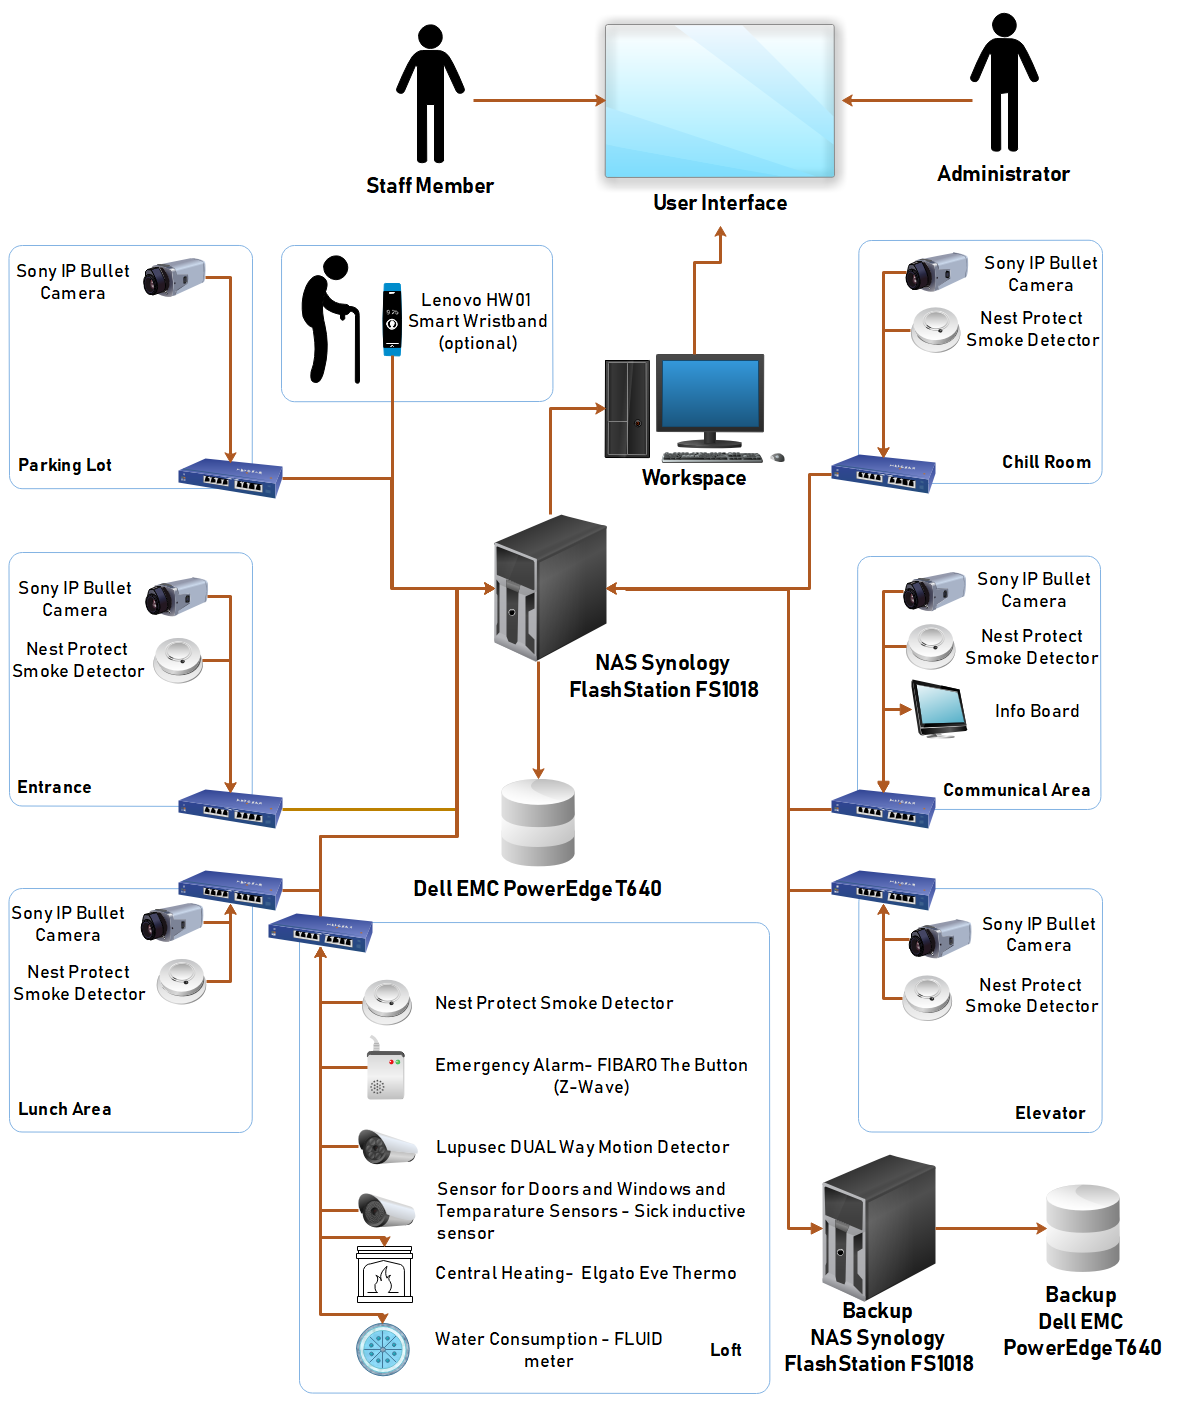
\includegraphics[width =1.0\textwidth]{images/architecture.PNG}
	\caption{Basic concept}
	\label{architecure}
\end{figure}
The figure shows the central hardware components of the iCare system and the connected devices. The rectangles represent the different rooms of the building. Each room has a HUB that communicates with the central server of the iCare system. In each room, the devices shown in the associated rectangle are installed as part of the iCare system, which communicate with the room's HUB via a wireless connection. This way, the required data reaches the server and is persisted in a database if required. The iCare server uses a RAID 2 backup system with a backup database to ensure the safety of the aquired data. The data can be accessed by employees or the administrator from any workspace using a web user-interface. The authorisation specified in the specification applies to the access to areas which show protected contents. In addition, patients can be given wristbands which monitor their vital functions on a voluntary basis or by order of a doctor. These wristbands communicate with the central server via a wireless connection and transmit the recorded data in real time.
\subsection{Project Managment Report [Prmr]}
\label{sec:orgd96ec13}
\begin{center}
\begin{tabular}{|l|r|}
	\hline
	 & Time in hours\\
	 \hline
	optimistic & 65\\
	\hline
	most likely & 92\\
	\hline
	pessimistic & 130\\
	\hline
\end{tabular}
\end{center}
\begin{itemize}
\item create product requirement catalog (50 / 70 / 100)
\item create GANTT diagram (5 /10 / 15)
\item negoitate time and costs with customer (10 / 12 /15 )
\end{itemize}

\subsection{Hardware prerequisites [Hpre]}
\label{sec:orgfb33f5b}

\begin{center}
	\begin{tabular}{|l|r|}
		\hline
		& Time in hours\\
		\hline
		optimistic & 108\\
		\hline
		most likely & 182\\
		\hline
		pessimistic & 256\\
		\hline
	\end{tabular}
\end{center}


\subsubsection{Video cameras [HpreCam]}
\label{sec:org3a27049}
	\begin{enumerate}
	\item research for good product
	\begin{itemize}
	\item investigate environment / areas / building (8/10/12)
	\item estimate amounts and total costs (8/10/12)
	\end{itemize}
	\item negotiate with customer (8/10/12)
	\item buy those products (8/10/12)
	\end{enumerate}

\subsubsection{Storage [HpreS]}
\label{sec:orgeb93f9e}
\begin{enumerate}
\item research archive backup file system
\begin{itemize}
\item NAS with redundance (RAID 2) (4/6/8)
\item Backup also with (RAID 2) (4/6/8)
\end{itemize}
\end{enumerate}

\subsubsection{Panels [HpreP]}
\label{sec:org4b41c6c}
\begin{enumerate}
\item research for good product
\begin{itemize}
\item investigate environment / areas / building (8/10/12)
\item estimate amounts and total costs (4/8/12)
\end{itemize}
\item negotiate with customer (4/8/12)
\item buy those products (4/8/12)
\end{enumerate}

\subsubsection{Control Unit (PLC) [HprePLC]}
\label{sec:orgd40ef86}
\begin{enumerate}
\item research for good product
\begin{itemize}
\item investigate environment / areas / building (4/8/12)
\item estimate amounts and total costs (4/8/12)
\end{itemize}
\item negotiate with customer (4/8/12)
\item buy those products (4/8/12)
\end{enumerate}

\subsubsection{Server [HpreSer]}
\label{sec:org7b31fb6}
\begin{enumerate}
\item research for good product
\begin{itemize}
\item investigate environment / areas / building (4/8/12)
\item estimate amounts and total costs (4/8/12)
\end{itemize}
\item negotiate with customer (4/8/12)
\item buy those products (4/8/12)
\end{enumerate}
\subsubsection{Sensors [HpreSens]}
\label{sec:org6352bec}

\begin{enumerate}
\item research for good product
\begin{itemize}
\item investigate environment / areas / building (4/8/12)
\item estimate amounts and total costs (4/8/12)
\end{itemize}
\item negotiate with customer (4/8/12)
\item buy those products (4/8/12)
\end{enumerate}



\subsection{Hardware installation [Hin]}
\label{sec:org2cae8f9}

\begin{center}
\begin{tabular}{|l|r|}
	\hline
	& Time in hours\\
	\hline
	optimistic & 40\\
	\hline
	most likely & 50\\
	\hline
	pessimistic & 60\\
	\hline
\end{tabular}
\end{center}

\subsubsection{installation and configuration}
\label{sec:org7c12187}
\begin{itemize}
\item video cameras (8/10/12) [HinCam] 
	\begin{itemize}
	\item dependent on [HpreCam]
	\end{itemize}
\item storage  (8/10/12)[HinS]
	\begin{itemize}
	\item dependent on [HpreS, HpreCam]
	\item connect video cameras to system
	\end{itemize}
\item panels (8/10/12)[HinP]
	\begin{itemize}
	\item dependent on [HpreP]
	\item configuration
	\end{itemize}
\item Control Unit (PLC) (8/10/12) [HinPLC]
	\begin{itemize}
	\item dependent on [HpreP]
	\end{itemize}
\item Sensors (8/10/12) [HinSens]
	\begin{itemize}
	\item dependent on [HpreSens]
	\end{itemize}
\end{itemize}

\subsection{Software prerequisites [Spre]}
\label{sec:org180caa5}

\begin{center}
\begin{tabular}{|l|r|}
	\hline
	& Time in hours\\
	\hline
	optimistic & 2\\
	\hline
	most likely & 8\\
	\hline
	pessimistic & 16\\
	\hline
\end{tabular}
\end{center}

\subsubsection{Matlab [SpreMat]}
\label{sec:orgda25cf6}
\begin{itemize}
\item Buy licence / install software  (1/4/8)
\end{itemize}

\subsubsection{PLC IDEs - Automation Studio [SprePLC]}
\label{sec:org003d4a8}
\begin{itemize}
\item Buy licence / install software (1/4/8)
\end{itemize}

\subsection{Software [So]}
\label{sec:orgdf36b5c}

\begin{center}
\begin{tabular}{|l|r|}
	\hline
	& Time in hours\\
	\hline
	optimistic & 604\\
	\hline
	most likely & 810\\
	\hline
	pessimistic & 1259\\
	\hline
\end{tabular}
\end{center}
\subsubsection{create infrastructure [SoInf]}
\label{sec:org06c00a2}
\begin{itemize}
\item setup wiki (1/4/8)
\item setup slack (1/2/3)
\item setup git respository (1/2/3)
\item setup task managment (1/2/3)
\end{itemize}
\subsubsection{System analysis [SoAn]}
\label{sec:org498acda}
\begin{itemize}
\item design architecture (24 / 30 / 48)
\item define components / communication with external systems (interfaces) (24 / 30 / 48)
\item invastigate time in finding out what technologies we want to use (24 / 30 / 48)
\item create diagrams(24 / 30 / 48)
\item describe behaviour of components and depedencies (24 / 30 / 48)
\item find out problematic and time consuming tasks and challanges (24 / 30 / 48)
\end{itemize}
\subsubsection{System design [SoDes]}
\label{sec:org1137d7c}
\begin{itemize}
\item design mutliple GUI and Usability concept (48 / 60 / 90 )
\item gather feedback from customer and redesign concepts (48 / 60 / 90 )
\item design prototyp with fake data (48 / 60 / 90 )
\end{itemize}
\subsubsection{System implementation [SoImpl]}
\label{sec:orgf2f809f}
\begin{itemize}
\item implement components (200 / 300 / 480)
\item unit tests (24 / 30 / 48)
\item integration test (24 / 30 / 48)
\item E2E testing (24 / 30 / 48)
\item documentation (40 / 50 / 60)
\end{itemize}



\subsection{Delivery [Dlvry]}
\label{sec:org1388080}
\begin{center}
\begin{tabular}{|l|r|}
	\hline
	& Time in hours\\
	\hline
	optimistic & 13\\
	\hline
	most likely & 30\\
	\hline
	pessimistic & 50\\
	\hline
\end{tabular}
\end{center}
\begin{itemize}
\item present / demonstrate system and software (12 / 20 / 30)
\item get customer approval (1 /10 / 20)
\end{itemize}

\subsection{Precedence Chart}
\begin{figure}[h]
	\centering
	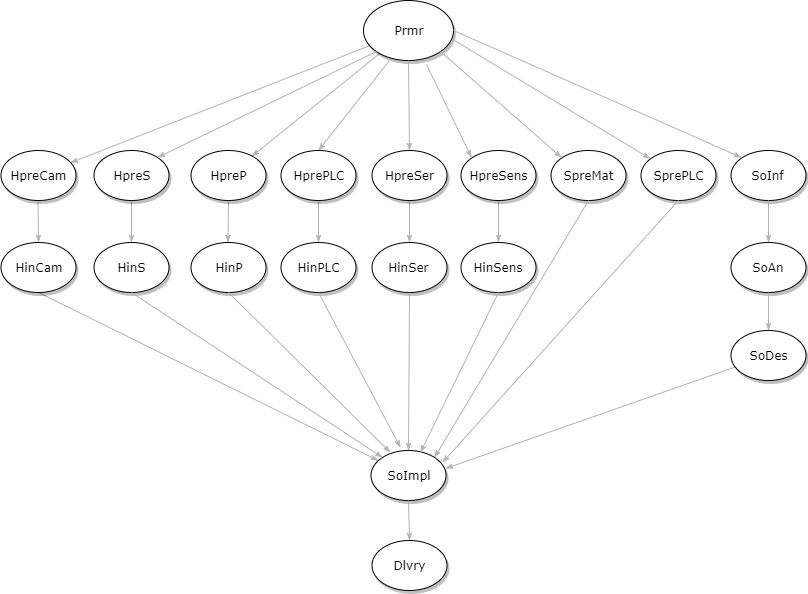
\includegraphics[width=\textwidth]{images/precedenceChart}
\end{figure}


\chapter{Product and Cost Analysis}
\label{market-analysis}
The Care Home is a facility that attaches great importance to safety and energy efficiency. Therefore, it is essential to check different products for certain characteristics. The following attributes are particularly important.
\begin{itemize}
	\item power consumption (sustainability)
	\item costs
	\item integration with systems
	\item compatibility
	\item maintainability
	\item lifespan
	\item customer support 
\end{itemize}

%=================================================================================
\section{Surveillance camera}
By taking the criteria into account, the closer decision was made on two models. The \textit{Bascom Pro Dom-Camera} and the \textit{Sony IP SNC-EB632R}. Dome cameras are semicircular and can be mounted on the ceiling or on a roof (as opposed to bullet cameras). Dome cameras also attract less attention. Bacom's Dome camera uses wireless data transmission and can be connected to the regular power supply. The Sony camera can be powered via Ethernet (power over ethernet) and also provides data via the same cable. Both have an IP66 standard. Thus they can be used inside as well as outside of the building. There is hardly any difference in price, which is why this does not contribute to the purchase decision. However, the wired version is more reliable as signal interference has less influence on the quality. Therefore, the first choice is the Sony camera.
\begin{figure}[h]% 
	\centering 
	\subfloat[Bascom Dome Camera]{ 
		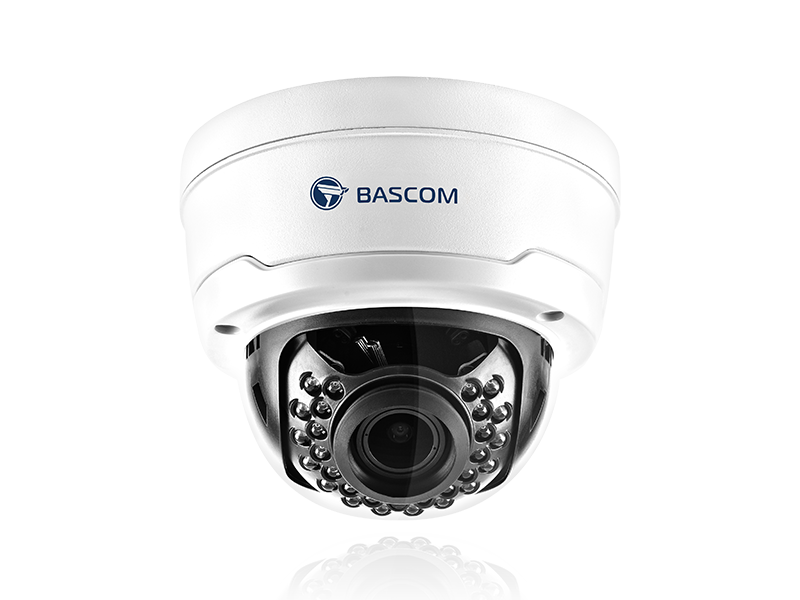
\includegraphics[width=0.4\textwidth]{images/CostAnalysis/domeCamera-pd20}% 
	} \hspace{1cm}
	\subfloat[Recorder for Dome Camera]{ 
		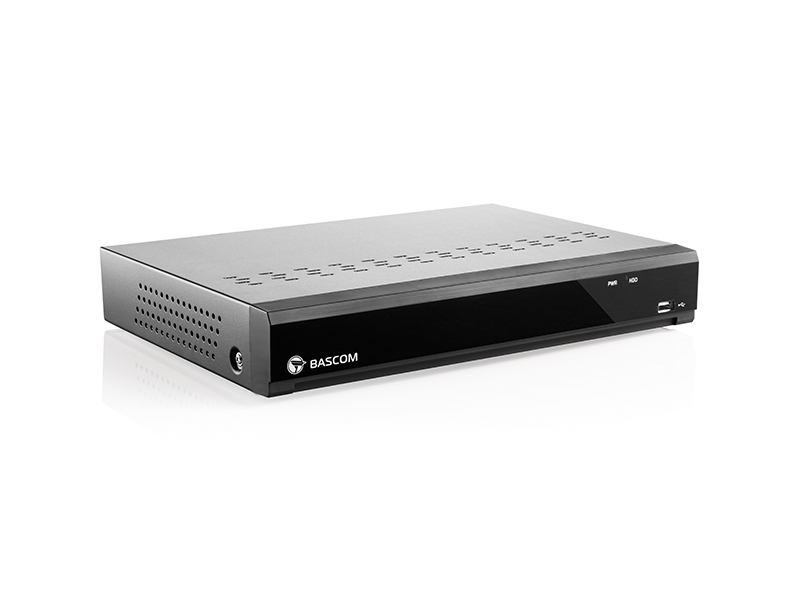
\includegraphics[width=0.4\textwidth]{images/CostAnalysis/recorder-pr4}% 
	} 
	\caption{Dome Camera System}% 
	\label{fig:domeCameraSystem}% 
\end{figure}

\begin{figure}[h]
	\centering
	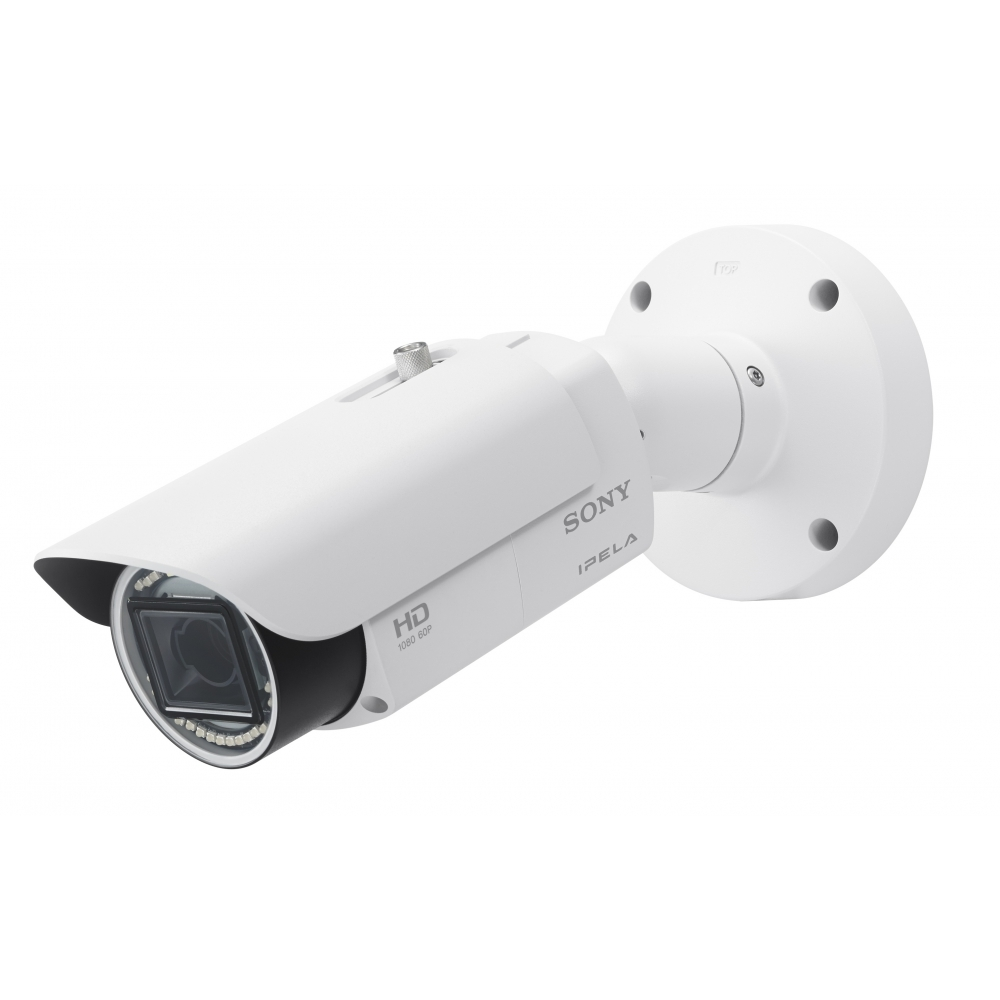
\includegraphics[width=.5\textwidth]{images/CostAnalysis/sony-ip-bullet-kamera} 
	\caption{Sony IP Bullet Camera}
	\label{fig:sonyCamera}
\end{figure}

%=================================================================================
\section{Smoke detector}
In the event of a fire, it is essential to have reliable smoke detectors in operation. Since this project aims to score points above all with customer satisfaction, inconspicuous and simple smoke detectors are preferable. There are several manufacturers that produce, for example, smart smoke detectors. Examples are Bosch, Nest or innogy. Smart devices have the advantage of being relatively easy to integrate into a system. The data can be retrieved via Wifi, Bluetooth or via web app. It is even possible to integrate the functions of the smoke detector into your own application via the API.
\\
Considering the above mentioned criteria, the choice was made for the second generation of the \textit{Nest Protect}. It scores with its simple appearance and the variety of functionality.  The price and performance of this device match very well and outperform the competition.

\begin{figure}[h]
	\centering
	
\includegraphics[width=.4\textwidth]{images/CostAnalysis/NestProtect} 
	\caption{Nest Protect Smoke Detector}
	\label{fig:smokeDetection}
\end{figure}

%=================================================================================
\section{NAS }
The network hard disk is a device that must function reliably. Important data is stored there and must be quickly accessible. That's why sufficient RAM (at least 8 GB) and a modern processor is of great importance. Another important point is of course the scalability, as well as the integration into the system, and commissioning.
\clearpage
\begin{figure}[h]
	\centering
	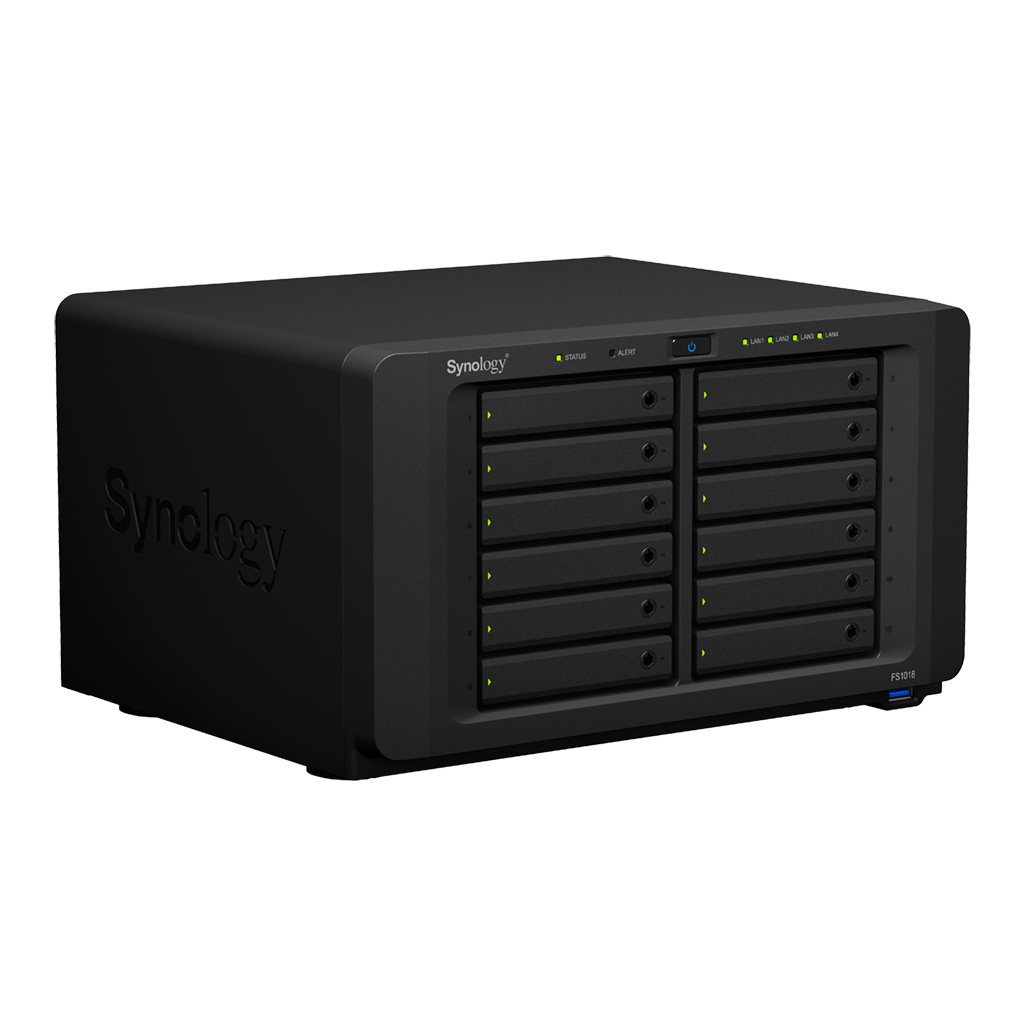
\includegraphics[width=.6\textwidth]{images/CostAnalysis/synologyFS1018} 
	\caption{NAS}
	\label{fig:nas}
\end{figure}

At this point, the \textit{Synology FlashStation FS1018} was chosen. With 12 SSD disks, it has sufficient storage capacity to store the most important data over a long period of time. The specifications are also appealing. Synology advertises their product with low latency, which is important for the application because emergency data, for example, must be retrieved quickly.

%=================================================================================
\section{Inductive and smart sensors}
In this application, inductive sensors are required to obtain the status of different furnishing objects. Examples of this are e. g. whether a door or a window is open or closed. Inductive sensors are available in different sizes, from different manufacturers. However, the choice fell on a certain sensor from Sick. The \textit{Sick IME08-1B5PSZT0S} is an inconspicuous and reliable proximity sensor that fits well into our concept. 
\newpage
\begin{figure}[h]
	\centering
	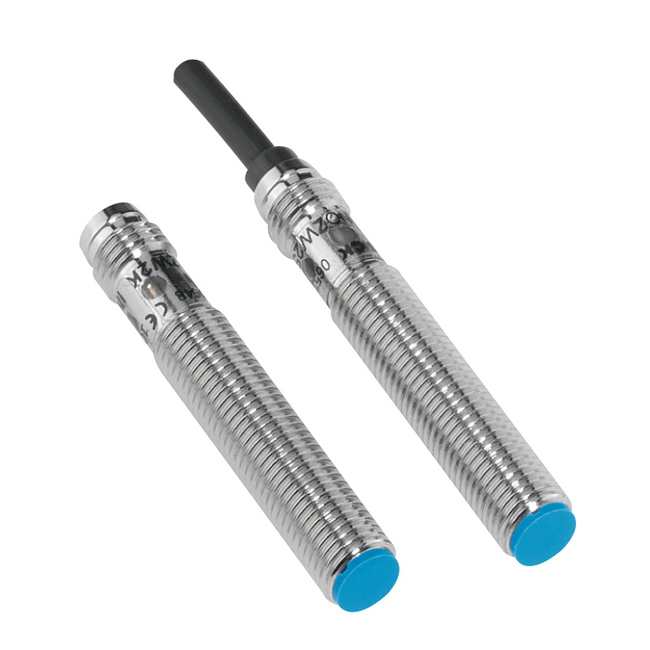
\includegraphics[width=.4\textwidth]{images/CostAnalysis/sickIni} 
	\caption{Sick inductive sensor}
	\label{fig:sickIni}
\end{figure}

Another idea is to use a smart sensor instead of an inductive sensor. The smart heating system (chapter \ref{sec:smartHeating}) enables these two systems to interact with each other in order to create an efficient cooperation. A certain smart door and window contact from Panasonic has stood out. The \textit{Panasonic KX-HNS101}.

\begin{figure}[h]
	\centering
	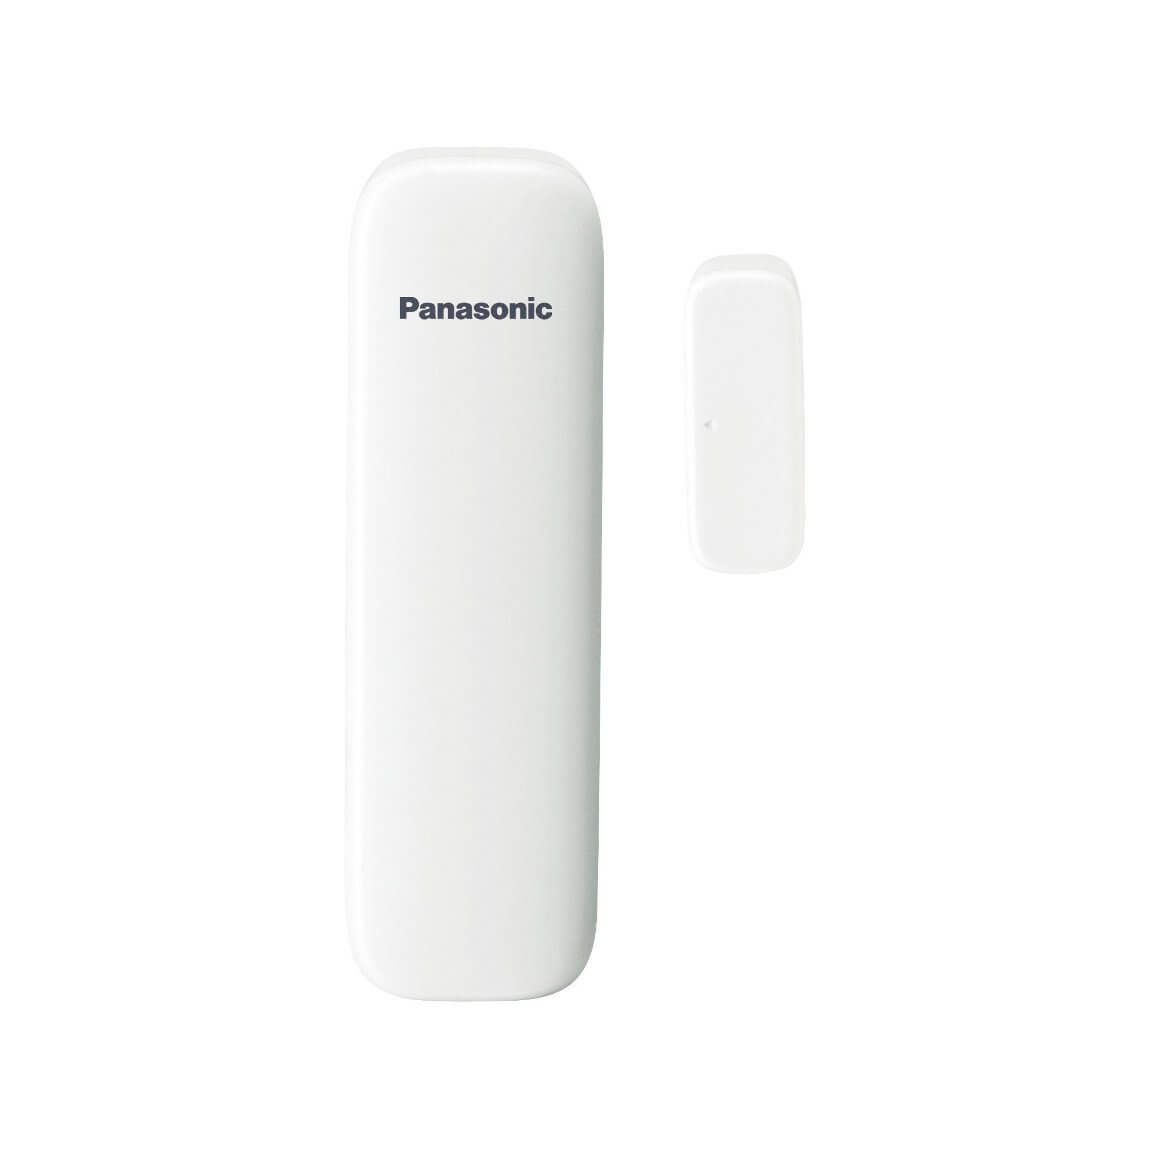
\includegraphics[width=.4\textwidth]{images/CostAnalysis/panasonicfensterkontakt} 
	\caption{Sick inductive sensor}
	\label{fig:panasonicSmart}
\end{figure}

%=================================================================================
\section{Database Server}
An important aspect of this project is the storage of data in a database. For this it is important that it is both scalable and robust. Data must be transported quickly and securely. And a lot of memory must be available. The \textit{Dell EMC PowerEdge T640} was selected for this. Because it is a tower server and not a server for the rack, the consumption is lower, which fits our needs for this project.

\begin{figure}[h]
	\centering
	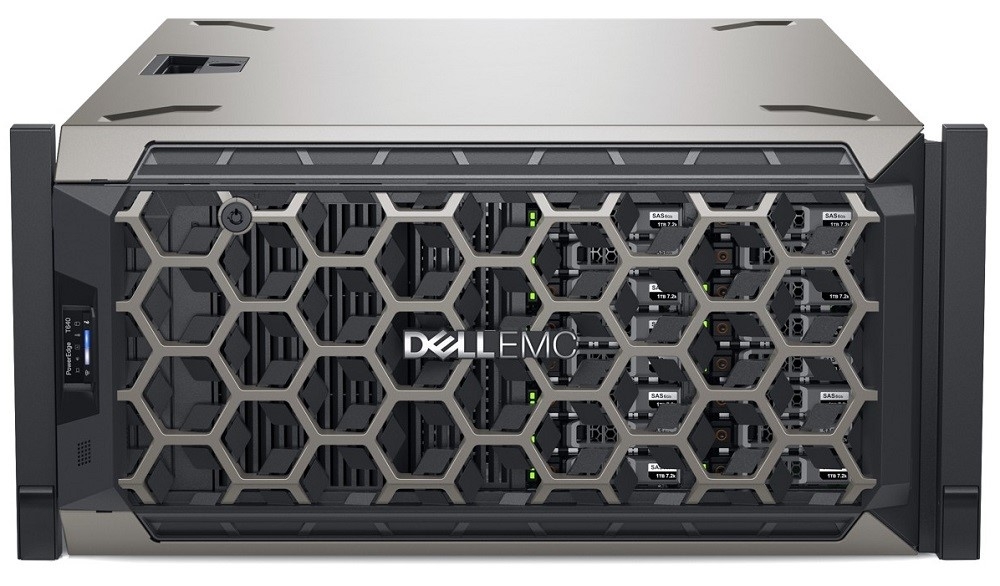
\includegraphics[width=.6\textwidth]{images/CostAnalysis/DellEMCPowerEdgeT640} 
	\caption{Dell EMC PowerEdge T640}
	\label{fig:dbServer}
\end{figure}

%=================================================================================
\section{CPU for PLC System}
PLC systems are used to process sensor data and send signals to devices. In this way, controllers can be written that receive, process sensor data and supply outputs that control actuators. This can be used to realize comfort functions. When a sensor receives a certain value, an actuator is activated which automatically opens doors or switches lights on or off, for example. Since we gained a lot of positive experience with B\&R through other projects, the choice was made for the \textit{X20CP1485 CPU}. It is characterised by its compact size, low energy consumption and extensibility. It is also capable of supporting various protocols such as POWERLINK or CAN. Thus we are flexible in development and can react dynamically to hardware changes.

\begin{figure}[h]
	\centering
	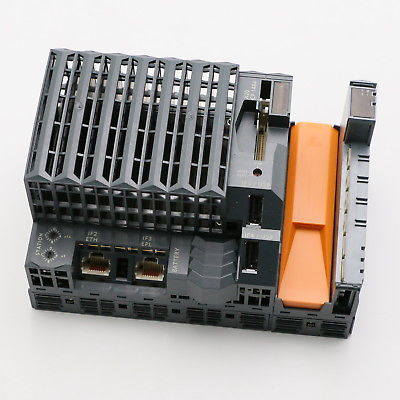
\includegraphics[width=.5\textwidth]{images/CostAnalysis/BR-Automation-X20-CP-1484} 
	\caption{B\&R CPU}
	\label{fig:brCPU}
\end{figure}

%=================================================================================
\section{Motion detectors}
Motion detectors are an important part of our application. Since mostly elderly people live in the care home, it is important that they come into contact with technical equipment as little as possible. This increases the comfort factor enormously. They do not have to deal with technical innovations, but can enjoy their stay. The motion detectors are required to control lights, for example, when a resident is in a certain area. Since we don't want the residents to feel observed, the motion detector must be very simple. It must not interfere with the environment or be technically impaired by the exterior. Since there are also many manufacturers with good equipment like Philips, Elgato or Lupusec, the choice is not easy. The price-performance ratio and simplicity are an important point. That's why we chose the \textit{Lupusec DUAL Way}.
\newpage
\begin{figure}[h]
	\centering
	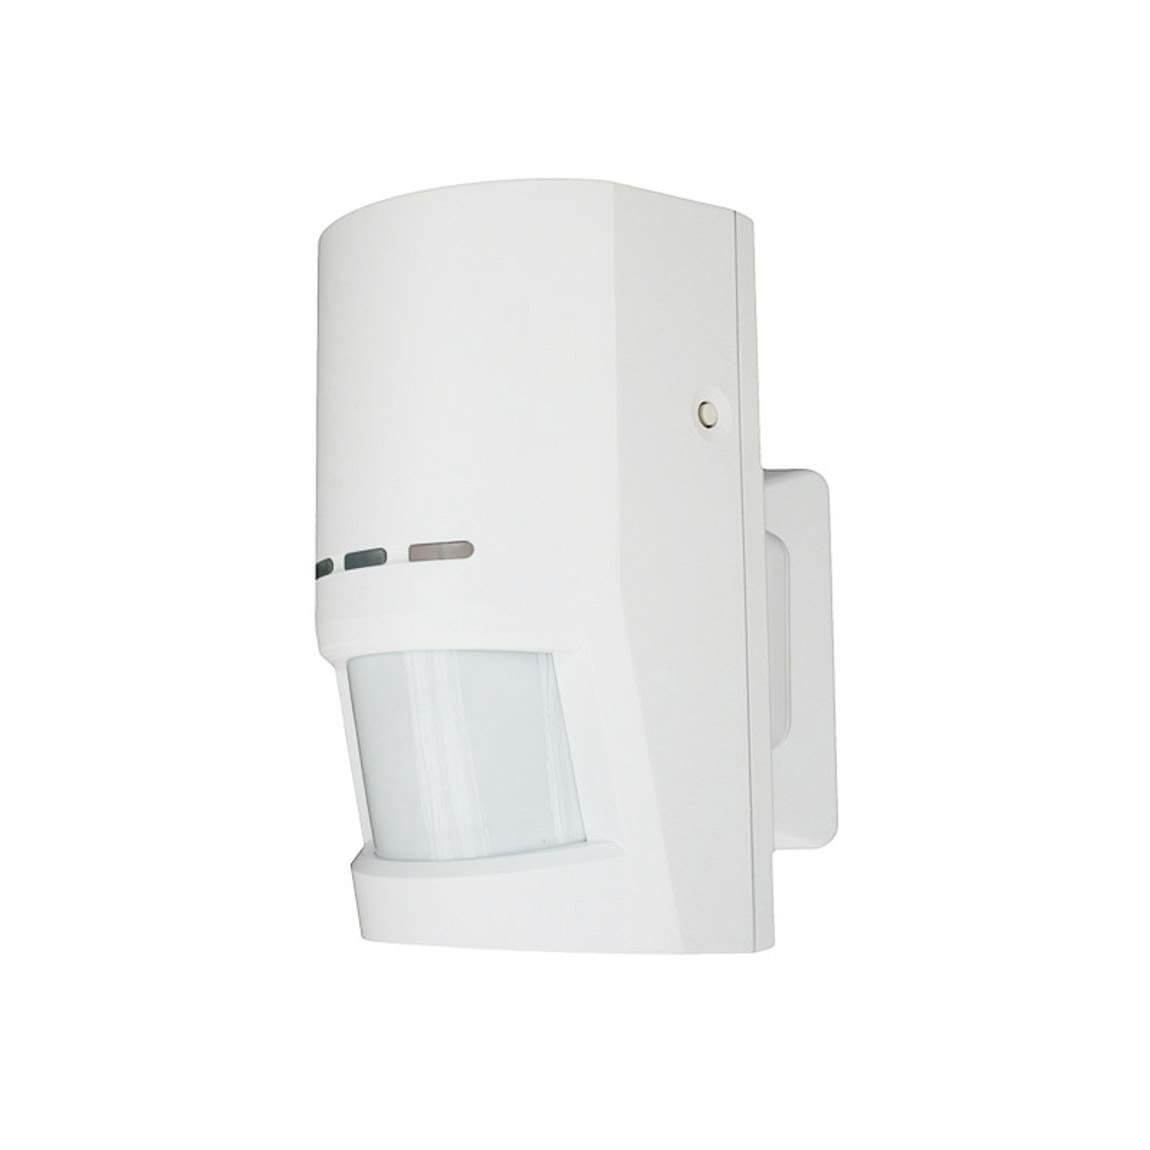
\includegraphics[width=.4\textwidth, trim=3cm 3cm 3cm 4cm, clip]{images/CostAnalysis/lupusecBewegungsmelder} 
	\caption{Lupusec DUAL Way}
	\label{fig:lupusecDual}
\end{figure}

%=================================================================================
\section{Healthcare Wristband}
A constant control of body values for patients can be very helpful to the caregivers. Classical methods such as pulse measurement or blood pressure measurement must be done manually by helpers and cost the patient time. During this time they are often not allowed to move, otherwise they can influence the values. Long-term measurements with old devices are complex and error-prone and do not give the patient a good and relaxing feeling. Our aim is to carry out long-term measurements, which the patient does not notice in the best case scenario. We use the \textit{Lenovo HW01 Smart Wristband}, which comes with a variety of features. 
\begin{itemize}
	\item pedometer
	\item sleep monitor
	\item heart rate measurement
	\item Date and time
	\item wake-up function
	\item stopwatch
	\item notifications
	\item Music playback control
	\item movement memory
	\item GPS run mode
\end{itemize}
Of course, this device does not replace special medical devices. However, it can be used for forecasting and unobtrusive monitoring, which can react quickly in an emergency.

\begin{figure}[h]
	\centering
	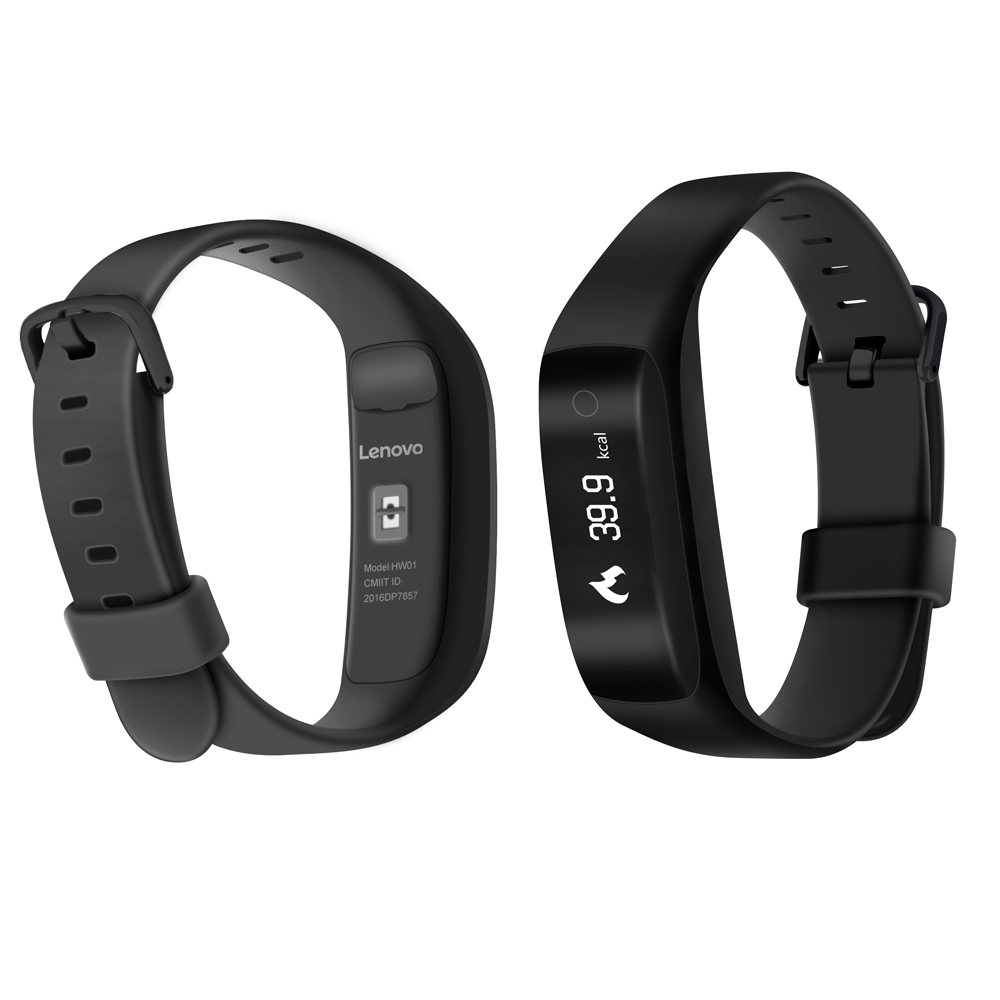
\includegraphics[width=.5\textwidth, trim=1cm 4cm 2cm 4cm, clip]{images/CostAnalysis/LenovoHW01} 
	\caption{Lenovo HW01 Smart Wristband}
	\label{fig:lenovoHealth}
\end{figure}

%=================================================================================
\section{Emergency button}
In order to offer patients the possibility to submit a message in case of emergency, we have decided to implement an emergency button. The data is then stored and evaluated centrally to prevent emergencies from being simulated or inadvertently activated. The \textit{FIBARO The Button (Z-Wave)} is a good and efficient way to realize this idea.
\newpage
\begin{figure}[h]
	\centering
	
\includegraphics[width=.4\textwidth]{images/CostAnalysis/fibaroEmergency} 
	\caption{FIBARO The Button (Z-Wave)}
	\label{fig:fibaroEmergency}
\end{figure}

%=================================================================================
\section{Smart heating system}
\label{sec:smartHeating}
A very important point in our product development is the heating of rooms. A lot of energy is lost there if the heating is not efficient. One of the market leaders in smart heating is the manufacturer Elgato. The product of our choice is the \textit{second-generation Elgato Eve Thermo}. 
\\
In addition to a simple installation, simple appearance and display, it comes with a variety of useful functions. Schedules can be set for heating schedules. It is also possible to view a consumption analysis. Both for the heating behaviour and for the energy. Another useful feature is the possibility to connect doors and window sensors with the smart heating system. As a result, the system knows when the windows and doors are opened and can regulate the heating process efficiently.
\newpage
\begin{figure}[h]
	\centering
	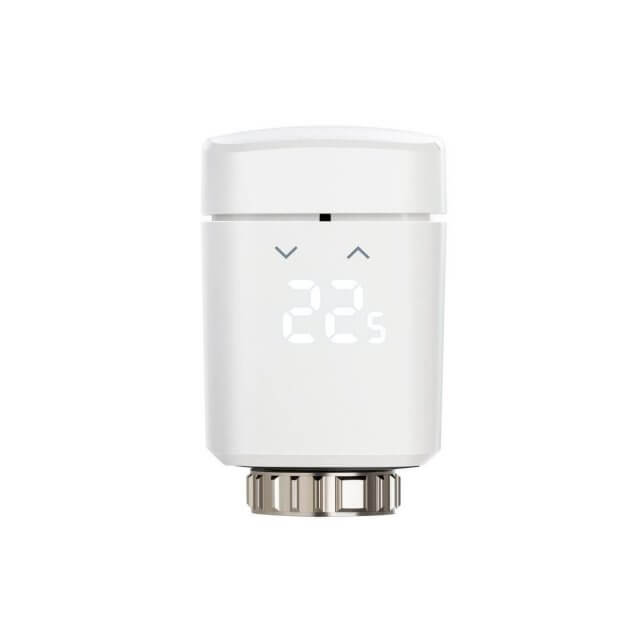
\includegraphics[width=.5\textwidth, trim=0 3cm 0 3cm, clip]{images/CostAnalysis/elgato-eve-thermo} 
	\caption{Elgato Eve Thermo}
	\label{fig:elgatoEve}
\end{figure}

%=================================================================================
\section{Water consumption}
A very important point in the care home system is the analysis and monitoring of water consumption. The data should be collected automatically and forwarded to a central point so that water consumption can be regulated. Abnormal behaviour can also be detected, for example, if someone has forgotten to turn off the water. In this case, warning signals can be sent to the staff to check that everything is in order and can act quickly in an emergency. A very interesting product is the \textit{FLUID meter}, which is used in our project.

\begin{figure}[h]
	\centering
	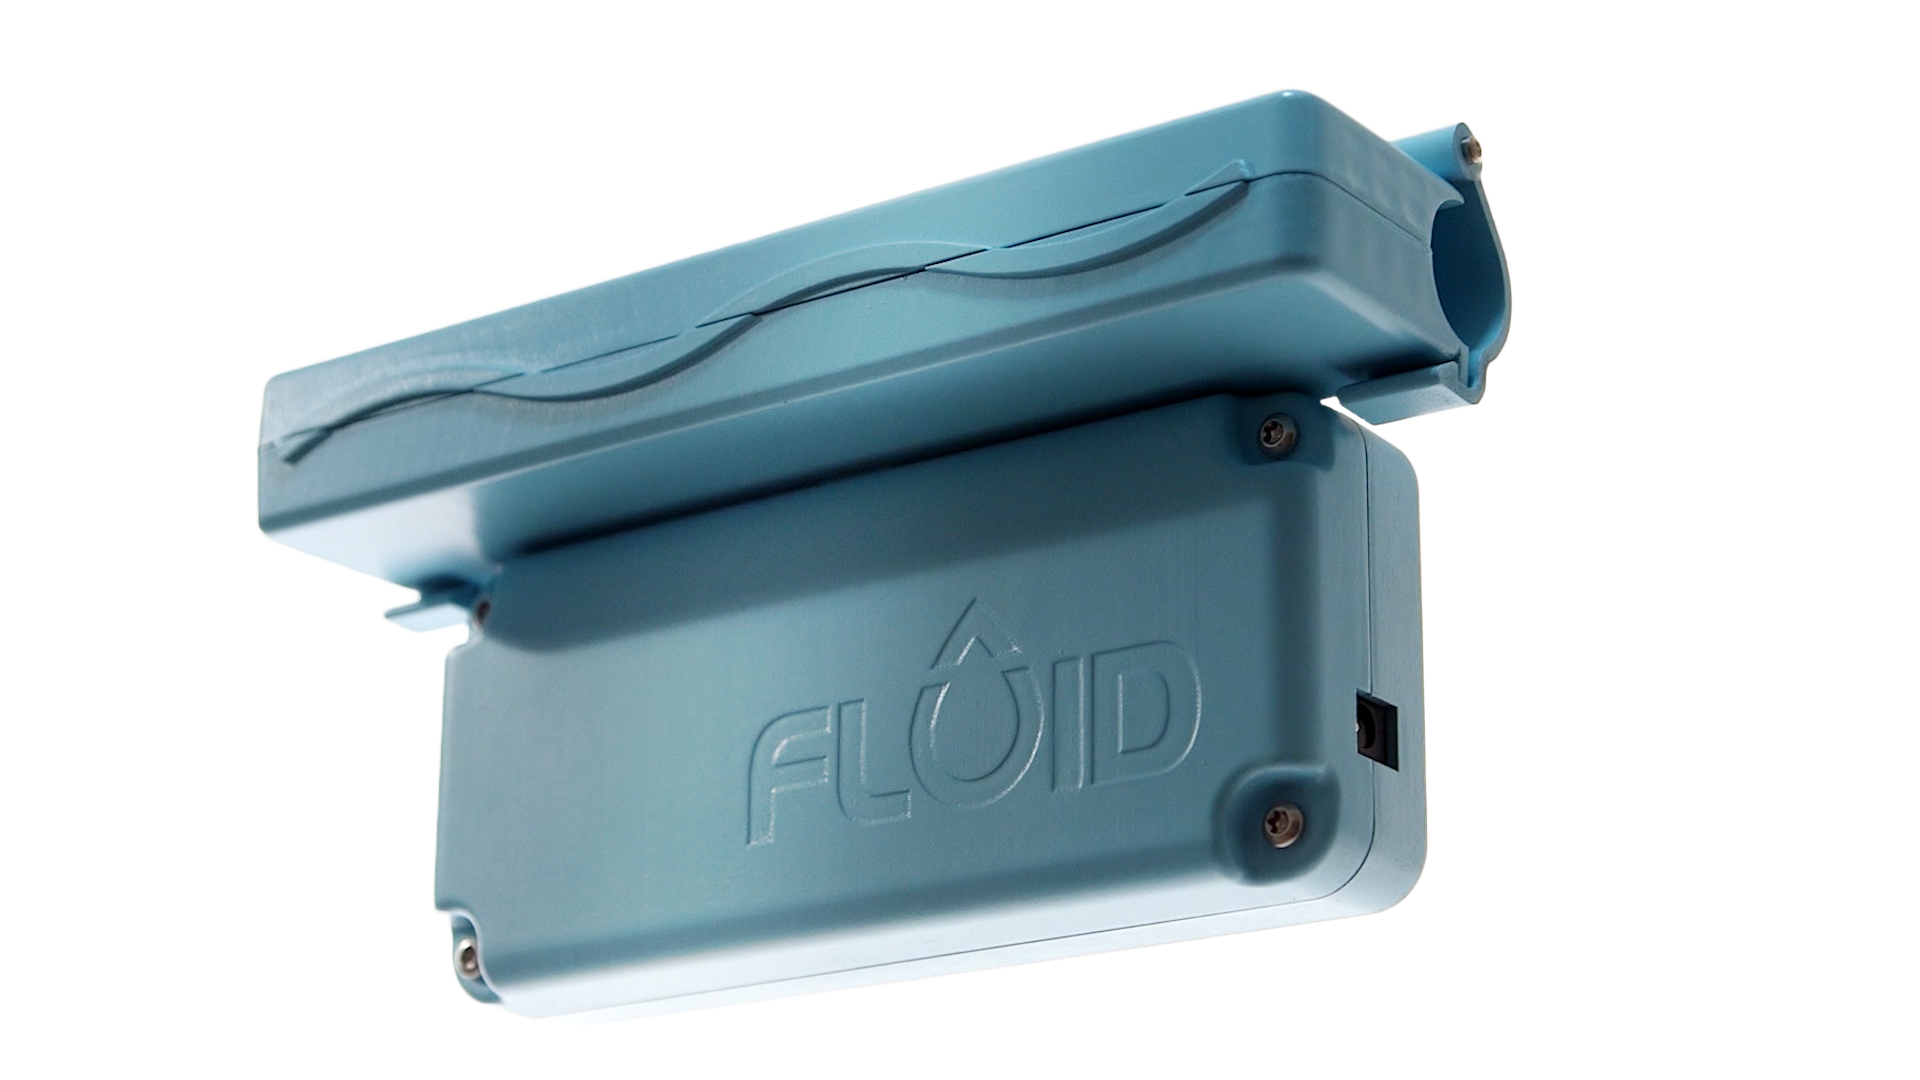
\includegraphics[width=.6\textwidth]{images/CostAnalysis/fluidMeter} 
	\caption[FLUID meter]{FLUID meter\protect\footnotemark}
	\label{fig:fluidMeter}
\end{figure}
\footnotetext{Source:\\http://www.fluidwatermeter.com/wp-content/uploads/2014/11/Fluid-Campaign.00\_00\_57\_18.Still002.png}
%=================================================================================
\section{HMI Tablets}
It makes sense to use a portable tablets to transfer information quickly to the staff. The idea is that nurses can digitally enter and retrieve patient records. With one click statistics about patients and rooms can be retrieved and managed. Another use case is that the cleaning staff has a possibility to document the cleaned rooms. Things like cleanliness or contamination can be noted. Our product of choice is the \textit{iPad Pro}, which scores points for its performance and simple appearance. Although it is more expensive than the competition, we have had good experiences with these tablets in the past, which has made our decision easier.
\\
\\
\begin{figure}[h]
	\centering
	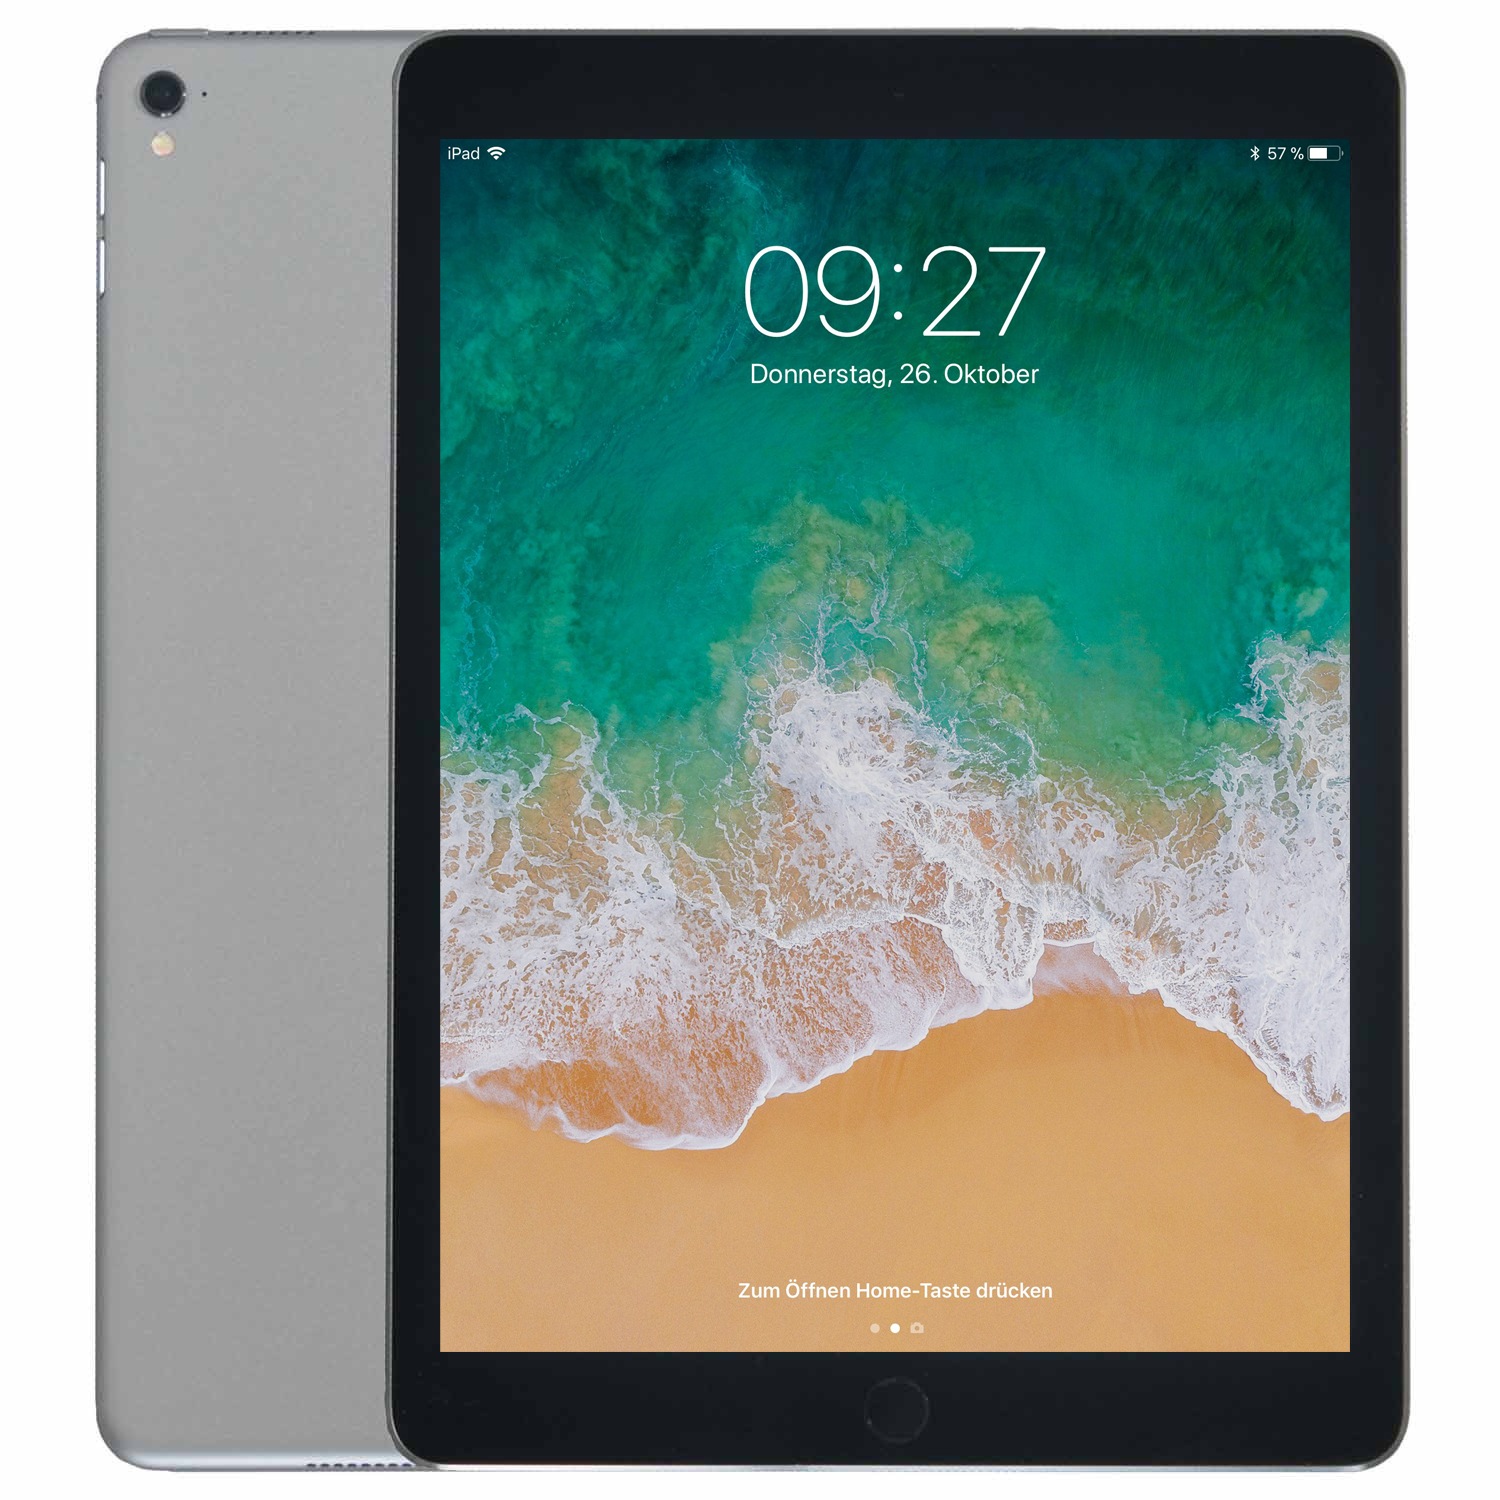
\includegraphics[width=.5\textwidth]{images/CostAnalysis/iPadPro} 
	\caption[12,9" iPad Pro]{12,9" iPad Pro\footnotemark}
	\label{fig:iPadPro}
\end{figure}
\footnotetext{Source: \\https://media.nbb-cdn.de/images/products/310000/316143/Apple\_iPadPro\_2017\_space\_Hero.jpg}
\clearpage
%=================================================================================
\section{Cost Calculation}
\begin{table}[h]
	\centering
	\renewcommand{\arraystretch}{1.9}
	\begin{tabular}{lrrr}
	Label & Price Per Unit [\officialeuro] & Amount & Cumulative Costs [\officialeuro] \\
	\hline
	Sony IP SNC-EB632R & 1,000 & 5 & 5,000\\
	Nest Protect & 130 & 120 & 15,600\\
	Synology FlashStation FS1018 & 1,600 & 2 & 3,200\\
	Panasonic KX-HNS101 & 30 & 250 & 7,500\\
	Dell EMC PowerEdge T640 & 2,000 & 2 & 4,000\\
	B\&R X20CP1485 & 2,000 & 2 & 4,000\\
	Lupusec DUAL Way & 200 & 160 & 32,000\\
	Lenovo HW01 Smart Wristband & 30 & 120 & 3,600\\
	FIBARO The Button (Z-Wave) & 50 & 110 & 5,500\\
	Elgato Eve Thermo 2. Gen & 80 & 110 & 8,800\\
	FLUID meter & 250 & 130 & 32,500\\
	12,9" iPad Pro & 1,000 & 20 & 20,000\\
	\hline
	%Products Total & & & \textbf{xxx}\\
	Working Hours (most likely)& 1172 & 100 & 117,200 \\
	Overhead Costs &  &  & 40,000\\
	\hline
	\hline
	Nett Total & & & 293,905\\
	+ VAT 20\% & & & 58,781\\
	\hline
	\hline
	\textbf{Total} & & & \textbf{352,686}
	\end{tabular}
\end{table}



% % %%%%%% Literaturverzeichnis (darf im deutschen nicht in den Anhang!)
% Einfaches Literaturverzeichnis
%\input{chapters/ch-zz-bibEinfach}
% Literaturverzeichnis mit Bibtex
%\Urlmuskip=0mu plus 1mu\relax
%\ihead[]{\leftmark} % links: Kapitel
%\chead[\pagemark]{\pagemark} % mitte:
%\ohead[]{} % rechts: Section
%\automark[]{chapter}
%\raggedright
%\sloppy
%\ihead[]{}
%\bibliographystyle{unsrt}
%\bibliography{bib/bib}

% % %%%%%% Anhang
%\appendix
%\include{chapters/ch-zz-anhang}

% %  Inhalt ENDE %%%%%%%%%%%%%%%%%%%%%%%%%%%%%%%%%%%%%%%%%%%%%%%%%%%%%%%%%%
\end{document}
